\documentclass[11pt]{article}
\usepackage[letterpaper,margin=.8in]{geometry}
% Shared font contract for manuscript text, math and figure labels.
% Matplotlib reads this preamble verbatim; do not use host-specific paths here.
\usepackage[T1]{fontenc}
\usepackage[utf8]{inputenc}
\usepackage{newtxtext,newtxmath}

\usepackage{graphicx,booktabs,array,amsmath,microtype,xurl}
\usepackage{placeins,caption}
\usepackage[numbers,sort&compress]{natbib}
\usepackage[hidelinks]{hyperref}
\usepackage{orcidlink}
\captionsetup{font=small,labelfont=normalfont,skip=5pt}
\setlength{\parskip}{.22em}
\setlength{\textfloatsep}{15pt plus 2pt minus 2pt}
\renewcommand{\topfraction}{.92}\renewcommand{\bottomfraction}{.88}\renewcommand{\textfraction}{.06}
\renewcommand{\floatpagefraction}{.8}
\makeatletter\setlength{\@fptop}{0pt}\let\tableinput\@@input\makeatother
\emergencystretch=2em\clubpenalty=10000\widowpenalty=10000
\graphicspath{{journal-figures/}}
\newcommand{\TotalObservations}{64,990}
\newcommand{\TotalLabelled}{63,685}
\newcommand{\TotalFrames}{29}
\newcommand{\PrimaryRuns}{351}
\newcommand{\TransferRuns}{45}
\newcommand{\NsclcDelta}{+0.097}
\newcommand{\NsclcLower}{+0.016}
\newcommand{\NsclcUpper}{+0.158}
\newcommand{\NsclcPca}{0.130}
\newcommand{\NsclcFull}{0.226}
\newcommand{\NsclcMean}{0.225}
\newcommand{\NsclcVsMean}{+0.002}
\newcommand{\NsclcVsMeanLower}{\ensuremath{-0.050}}
\newcommand{\NsclcVsMeanUpper}{+0.039}
\newcommand{\BccDelta}{\ensuremath{-0.026}}
\newcommand{\BccLower}{\ensuremath{-0.044}}
\newcommand{\BccUpper}{\ensuremath{-0.008}}
\newcommand{\BccPca}{0.168}
\newcommand{\BccFull}{0.141}
\newcommand{\BccMean}{0.149}
\newcommand{\BccVsMean}{\ensuremath{-0.008}}
\newcommand{\BccVsMeanLower}{\ensuremath{-0.037}}
\newcommand{\BccVsMeanUpper}{+0.028}
\newcommand{\BreastPca}{0.221}
\newcommand{\BreastFull}{0.154}
\newcommand{\BreastMean}{0.198}
\newcommand{\BreastNoContrast}{0.202}
\newcommand{\BreastDelta}{\ensuremath{-0.067}}
\newcommand{\TvaPca}{0.094}
\newcommand{\TvaFull}{0.149}
\newcommand{\TvaMean}{0.114}
\newcommand{\TvaNoContrast}{0.103}
\newcommand{\TvaDelta}{+0.056}
\newcommand{\HnsccPca}{0.271}
\newcommand{\HnsccFull}{0.219}
\newcommand{\HnsccMean}{0.211}
\newcommand{\HnsccNoContrast}{0.233}
\newcommand{\HnsccDelta}{\ensuremath{-0.052}}
\newcommand{\MibiPca}{0.210}
\newcommand{\MibiFull}{0.185}
\newcommand{\MibiMean}{0.149}
\newcommand{\MibiNoContrast}{0.209}
\newcommand{\MibiDelta}{\ensuremath{-0.025}}
\newcommand{\PositiveObjects}{5}
\newcommand{\NegativeObjects}{8}
\newcommand{\ContrastHelpsObjects}{5}
\newcommand{\ContrastHurtsObjects}{8}
\newcommand{\RegionTransferPcaAcc}{0.303}
\newcommand{\RegionTransferPcaBalanced}{0.257}
\newcommand{\RegionTransferSelfAcc}{0.336}
\newcommand{\RegionTransferSelfBalanced}{0.258}
\newcommand{\RegionTransferFullAcc}{0.382}
\newcommand{\RegionTransferFullBalanced}{0.312}
\newcommand{\CellTransferPcaAcc}{0.417}
\newcommand{\CellTransferPcaBalanced}{0.331}
\newcommand{\CellTransferSelfAcc}{0.400}
\newcommand{\CellTransferSelfBalanced}{0.326}
\newcommand{\CellTransferFullAcc}{0.339}
\newcommand{\CellTransferFullBalanced}{0.218}
\newcommand{\FullPeakMemory}{0.85}
\newcommand{\FullTimeMin}{0.78}
\newcommand{\FullTimeMax}{1.85}

\newcommand{\BccCommonKBetter}{2}
\newcommand{\BccCommonKDelta}{\ensuremath{-0.012}}
\newcommand{\BccNestedControlMean}{0.177}
\newcommand{\BccNestedDelta}{\ensuremath{-0.035}}
\newcommand{\BccNestedMax}{\ensuremath{-0.016}}
\newcommand{\BccNestedMin}{\ensuremath{-0.067}}
\newcommand{\BccNestedP}{0.125}
\newcommand{\BccNestedTesseraBetter}{0}
\newcommand{\BccVsPcaP}{0.125}
\newcommand{\BccVsPcaPositive}{0}
\newcommand{\BccWholeVsControlBetter}{0}
\newcommand{\BccWholeVsControlMean}{\ensuremath{-0.022}}
\newcommand{\BccWholeVsControlP}{0.125}
\newcommand{\BccWholeVsPcaMean}{\ensuremath{-0.025}}
\newcommand{\BccWholeVsPcaP}{0.125}
\newcommand{\BccWholeVsPcaPositive}{0}
\newcommand{\BelowSelfOnly}{8}
\newcommand{\CellTypeMean}{0.093}
\newcommand{\CellTypePca}{0.192}
\newcommand{\CellTypeTessera}{0.151}
\newcommand{\CellTypeTesseraLower}{4}
\newcommand{\GateAurocMax}{0.621}
\newcommand{\GateAurocMedian}{0.495}
\newcommand{\GateAurocMin}{0.385}
\newcommand{\GateBeaten}{12}
\newcommand{\GateExprAurocMedian}{0.536}
\newcommand{\GateObjects}{13}
\newcommand{\LungCommonKBetter}{5}
\newcommand{\LungCommonKDelta}{+0.166}
\newcommand{\LungGateLowMax}{81}
\newcommand{\LungGateLowMin}{50}
\newcommand{\LungGateMedianMax}{0.091}
\newcommand{\LungGateMedianMin}{0.011}
\newcommand{\LungNestedControlMean}{0.392}
\newcommand{\LungNestedDelta}{\ensuremath{-0.166}}
\newcommand{\LungNestedMax}{\ensuremath{-0.110}}
\newcommand{\LungNestedMin}{\ensuremath{-0.247}}
\newcommand{\LungNestedP}{0.0625}
\newcommand{\LungNestedTesseraBetter}{0}
\newcommand{\LungVsPcaP}{0.125}
\newcommand{\LungVsPcaPositive}{4}
\newcommand{\LungWeightTvdMax}{0.407}
\newcommand{\LungWeightTvdMin}{0.318}
\newcommand{\LungWholeVsControlBetter}{0}
\newcommand{\LungWholeVsControlMean}{\ensuremath{-0.147}}
\newcommand{\LungWholeVsControlP}{0.0625}
\newcommand{\LungWholeVsPcaMean}{+0.058}
\newcommand{\LungWholeVsPcaP}{0.188}
\newcommand{\LungWholeVsPcaPositive}{4}
\newcommand{\NoContrastSelfMaxGap}{0.004}
\newcommand{\NoGateAtLeast}{5}
\newcommand{\NoGateMean}{+0.019}
\newcommand{\PermNoContrastMaxGap}{0.004}
\newcommand{\StabilityPcaMin}{0.57}
\newcommand{\StabilityTesseraMax}{0.73}
\newcommand{\StabilityTesseraMin}{0.38}
\newcommand{\TransferCellFull}{0.218}
\newcommand{\TransferCellMeanSix}{0.096}
\newcommand{\TransferCellMeanTwoHundred}{0.072}
\newcommand{\TransferCellPca}{0.331}
\newcommand{\TransferCellTesseraBelowPca}{5}
\newcommand{\TransferRegionFull}{0.312}
\newcommand{\TransferRegionMeanSix}{0.297}
\newcommand{\TransferRegionMeanTwoHundred}{0.349}
\newcommand{\TransferRegionPca}{0.257}
\newcommand{\TransferRegionTesseraBelowPca}{0}
\newcommand{\WholeCellsMax}{100,335}
\newcommand{\WholeCellsMin}{21,368}

\newcommand{\BrCortexBestK}{200}
\newcommand{\BrCortexContig}{0.905}
\newcommand{\BrCortexGate}{0.457}
\newcommand{\BrCortexMean}{0.253}
\newcommand{\BrCortexNested}{0.286}
\newcommand{\BrCortexOracle}{0.341}
\newcommand{\BrCortexPca}{0.190}
\newcommand{\BrCortexTess}{0.416}
\newcommand{\BrCortexTessNested}{+0.131}
\newcommand{\BrCortexTessOracle}{+0.075}
\newcommand{\BrCortexTessPca}{+0.226}
\newcommand{\BrGateMax}{0.480}
\newcommand{\BrGateMin}{0.457}
\newcommand{\BrMerfishBestK}{100}
\newcommand{\BrMerfishContig}{0.931}
\newcommand{\BrMerfishGate}{0.468}
\newcommand{\BrMerfishMean}{0.175}
\newcommand{\BrMerfishNested}{0.425}
\newcommand{\BrMerfishOracle}{0.460}
\newcommand{\BrMerfishPca}{0.079}
\newcommand{\BrMerfishTess}{0.357}
\newcommand{\BrMerfishTessNested}{\ensuremath{-0.068}}
\newcommand{\BrMerfishTessOracle}{\ensuremath{-0.104}}
\newcommand{\BrMerfishTessPca}{+0.278}
\newcommand{\BrPcaGainMax}{0.342}
\newcommand{\BrPcaGainMin}{0.226}
\newcommand{\BrStarmapBestK}{30}
\newcommand{\BrStarmapContig}{0.921}
\newcommand{\BrStarmapGate}{0.480}
\newcommand{\BrStarmapMean}{0.491}
\newcommand{\BrStarmapNested}{0.568}
\newcommand{\BrStarmapOracle}{0.606}
\newcommand{\BrStarmapPca}{0.163}
\newcommand{\BrStarmapTess}{0.505}
\newcommand{\BrStarmapTessNested}{\ensuremath{-0.063}}
\newcommand{\BrStarmapTessOracle}{\ensuremath{-0.101}}
\newcommand{\BrStarmapTessPca}{+0.342}
\newcommand{\DevAllThirteenECoordMean}{+0.114}
\newcommand{\DevAllThirteenECoordNeg}{1}
\newcommand{\DevAllThirteenECoordP}{0.000488}
\newcommand{\DevAllThirteenECoordPos}{12}
\newcommand{\DevAllThirteenEMeanMean}{\ensuremath{-0.001}}
\newcommand{\DevAllThirteenEMeanNeg}{6}
\newcommand{\DevAllThirteenEMeanP}{0.835}
\newcommand{\DevAllThirteenEMeanPos}{7}
\newcommand{\DevAllThirteenEShufMean}{\ensuremath{-0.002}}
\newcommand{\DevAllThirteenEShufNeg}{7}
\newcommand{\DevAllThirteenEShufP}{0.664}
\newcommand{\DevAllThirteenEShufPos}{6}
\newcommand{\DevBccECoordMean}{+0.096}
\newcommand{\DevBccECoordNeg}{0}
\newcommand{\DevBccECoordP}{0.125}
\newcommand{\DevBccECoordPos}{4}
\newcommand{\DevBccEMeanMean}{\ensuremath{-0.006}}
\newcommand{\DevBccEMeanNeg}{3}
\newcommand{\DevBccEMeanP}{0.25}
\newcommand{\DevBccEMeanPos}{1}
\newcommand{\DevBccEShufMean}{\ensuremath{-0.009}}
\newcommand{\DevBccEShufNeg}{2}
\newcommand{\DevBccEShufP}{0.5}
\newcommand{\DevBccEShufPos}{2}
\newcommand{\DevLungECoordMean}{+0.100}
\newcommand{\DevLungECoordNeg}{1}
\newcommand{\DevLungECoordP}{0.125}
\newcommand{\DevLungECoordPos}{4}
\newcommand{\DevLungEMeanMean}{+0.001}
\newcommand{\DevLungEMeanNeg}{3}
\newcommand{\DevLungEMeanP}{0.938}
\newcommand{\DevLungEMeanPos}{2}
\newcommand{\DevLungEShufMean}{+0.002}
\newcommand{\DevLungEShufNeg}{3}
\newcommand{\DevLungEShufP}{0.875}
\newcommand{\DevLungEShufPos}{2}
\newcommand{\DevOthECoordMean}{+0.148}
\newcommand{\DevOthECoordNeg}{0}
\newcommand{\DevOthECoordP}{0.125}
\newcommand{\DevOthECoordPos}{4}
\newcommand{\DevOthEMeanMean}{+0.004}
\newcommand{\DevOthEMeanNeg}{0}
\newcommand{\DevOthEMeanP}{0.125}
\newcommand{\DevOthEMeanPos}{4}
\newcommand{\DevOthEShufMean}{+0.001}
\newcommand{\DevOthEShufNeg}{2}
\newcommand{\DevOthEShufP}{0.875}
\newcommand{\DevOthEShufPos}{2}
\newcommand{\HerAllECoordHi}{+0.261}
\newcommand{\HerAllECoordLo}{+0.120}
\newcommand{\HerAllECoordMean}{+0.194}
\newcommand{\HerAllECoordNeg}{0}
\newcommand{\HerAllECoordP}{0.00781}
\newcommand{\HerAllECoordPos}{8}
\newcommand{\HerAllENestedHi}{+0.053}
\newcommand{\HerAllENestedLo}{+0.004}
\newcommand{\HerAllENestedMean}{+0.027}
\newcommand{\HerAllENestedNeg}{2}
\newcommand{\HerAllENestedP}{0.0781}
\newcommand{\HerAllENestedPos}{6}
\newcommand{\HerAllEShufHi}{+0.015}
\newcommand{\HerAllEShufLo}{\ensuremath{-0.006}}
\newcommand{\HerAllEShufMean}{+0.005}
\newcommand{\HerAllEShufNeg}{2}
\newcommand{\HerAllEShufP}{0.469}
\newcommand{\HerAllEShufPos}{6}
\newcommand{\HerAllEUSixHi}{+0.011}
\newcommand{\HerAllEUSixLo}{\ensuremath{-0.005}}
\newcommand{\HerAllEUSixMean}{+0.003}
\newcommand{\HerAllEUSixNeg}{3}
\newcommand{\HerAllEUSixP}{0.438}
\newcommand{\HerAllEUSixPos}{5}
\newcommand{\HerAllTessNestedHi}{+0.002}
\newcommand{\HerAllTessNestedLo}{\ensuremath{-0.047}}
\newcommand{\HerAllTessNestedMean}{\ensuremath{-0.022}}
\newcommand{\HerAllTessNestedNeg}{6}
\newcommand{\HerAllTessNestedP}{0.141}
\newcommand{\HerAllTessNestedPos}{2}
\newcommand{\HerAllTessPcaHi}{+0.021}
\newcommand{\HerAllTessPcaLo}{\ensuremath{-0.053}}
\newcommand{\HerAllTessPcaMean}{\ensuremath{-0.015}}
\newcommand{\HerAllTessPcaNeg}{6}
\newcommand{\HerAllTessPcaP}{0.461}
\newcommand{\HerAllTessPcaPos}{2}
\newcommand{\HerAllTessUSixHi}{\ensuremath{-0.020}}
\newcommand{\HerAllTessUSixLo}{\ensuremath{-0.074}}
\newcommand{\HerAllTessUSixMean}{\ensuremath{-0.047}}
\newcommand{\HerAllTessUSixNeg}{7}
\newcommand{\HerAllTessUSixP}{0.0156}
\newcommand{\HerAllTessUSixPos}{1}
\newcommand{\HerAllUSixNestedHi}{+0.047}
\newcommand{\HerAllUSixNestedLo}{+0.004}
\newcommand{\HerAllUSixNestedMean}{+0.024}
\newcommand{\HerAllUSixNestedNeg}{2}
\newcommand{\HerAllUSixNestedP}{0.0781}
\newcommand{\HerAllUSixNestedPos}{6}
\newcommand{\HerBndECoordHi}{+0.456}
\newcommand{\HerBndECoordLo}{+0.157}
\newcommand{\HerBndECoordMean}{+0.309}
\newcommand{\HerBndECoordNeg}{0}
\newcommand{\HerBndECoordP}{0.00781}
\newcommand{\HerBndECoordPos}{8}
\newcommand{\HerBndENestedHi}{+0.074}
\newcommand{\HerBndENestedLo}{+0.009}
\newcommand{\HerBndENestedMean}{+0.042}
\newcommand{\HerBndENestedNeg}{1}
\newcommand{\HerBndENestedP}{0.0547}
\newcommand{\HerBndENestedPos}{7}
\newcommand{\HerBndEShufHi}{+0.016}
\newcommand{\HerBndEShufLo}{\ensuremath{-0.025}}
\newcommand{\HerBndEShufMean}{\ensuremath{-0.003}}
\newcommand{\HerBndEShufNeg}{4}
\newcommand{\HerBndEShufP}{0.805}
\newcommand{\HerBndEShufPos}{4}
\newcommand{\HerBndEUSixHi}{+0.005}
\newcommand{\HerBndEUSixLo}{\ensuremath{-0.029}}
\newcommand{\HerBndEUSixMean}{\ensuremath{-0.012}}
\newcommand{\HerBndEUSixNeg}{4}
\newcommand{\HerBndEUSixP}{0.258}
\newcommand{\HerBndEUSixPos}{4}
\newcommand{\HerBndGateAboveChance}{4}
\newcommand{\HerBndGateOverRaw}{4}
\newcommand{\HerBndSeamGate}{0.505}
\newcommand{\HerBndSeamGateHi}{0.544}
\newcommand{\HerBndSeamGateLo}{0.462}
\newcommand{\HerBndSeamPlain}{0.568}
\newcommand{\HerBndSeamPlainHi}{0.629}
\newcommand{\HerBndSeamPlainLo}{0.504}
\newcommand{\HerBndSeamRaw}{0.520}
\newcommand{\HerBndSeamRawGateHi}{+0.049}
\newcommand{\HerBndSeamRawGateLo}{\ensuremath{-0.017}}
\newcommand{\HerBndSeamRawGateMean}{+0.016}
\newcommand{\HerBndSeamRawGateNeg}{4}
\newcommand{\HerBndSeamRawGateP}{0.398}
\newcommand{\HerBndSeamRawGatePos}{4}
\newcommand{\HerBndSeamRawHi}{0.583}
\newcommand{\HerBndSeamRawLo}{0.453}
\newcommand{\HerBndSeamSmooth}{0.583}
\newcommand{\HerBndSeamSmoothGateHi}{+0.118}
\newcommand{\HerBndSeamSmoothGateLo}{+0.037}
\newcommand{\HerBndSeamSmoothGateMean}{+0.078}
\newcommand{\HerBndSeamSmoothGateNeg}{1}
\newcommand{\HerBndSeamSmoothGateP}{0.0156}
\newcommand{\HerBndSeamSmoothGatePos}{7}
\newcommand{\HerBndSeamSmoothHi}{0.650}
\newcommand{\HerBndSeamSmoothLo}{0.513}
\newcommand{\HerBndSeamSmoothPlainHi}{+0.023}
\newcommand{\HerBndSeamSmoothPlainLo}{+0.007}
\newcommand{\HerBndSeamSmoothPlainMean}{+0.015}
\newcommand{\HerBndSeamSmoothPlainNeg}{1}
\newcommand{\HerBndSeamSmoothPlainP}{0.0156}
\newcommand{\HerBndSeamSmoothPlainPos}{7}
\newcommand{\HerBndSeamSmoothRawHi}{+0.100}
\newcommand{\HerBndSeamSmoothRawLo}{+0.025}
\newcommand{\HerBndSeamSmoothRawMean}{+0.063}
\newcommand{\HerBndSeamSmoothRawNeg}{1}
\newcommand{\HerBndSeamSmoothRawP}{0.0234}
\newcommand{\HerBndSeamSmoothRawPos}{7}
\newcommand{\HerBndTessNestedHi}{+0.059}
\newcommand{\HerBndTessNestedLo}{\ensuremath{-0.080}}
\newcommand{\HerBndTessNestedMean}{\ensuremath{-0.008}}
\newcommand{\HerBndTessNestedNeg}{4}
\newcommand{\HerBndTessNestedP}{0.836}
\newcommand{\HerBndTessNestedPos}{4}
\newcommand{\HerBndTessPcaHi}{+0.068}
\newcommand{\HerBndTessPcaLo}{\ensuremath{-0.064}}
\newcommand{\HerBndTessPcaMean}{\ensuremath{-0.000}}
\newcommand{\HerBndTessPcaNeg}{5}
\newcommand{\HerBndTessPcaP}{1}
\newcommand{\HerBndTessPcaPos}{3}
\newcommand{\HerBndTessUSixHi}{\ensuremath{-0.000}}
\newcommand{\HerBndTessUSixLo}{\ensuremath{-0.132}}
\newcommand{\HerBndTessUSixMean}{\ensuremath{-0.062}}
\newcommand{\HerBndTessUSixNeg}{5}
\newcommand{\HerBndTessUSixP}{0.133}
\newcommand{\HerBndTessUSixPos}{3}
\newcommand{\HerBndThreeECoordHi}{+0.479}
\newcommand{\HerBndThreeECoordLo}{+0.160}
\newcommand{\HerBndThreeECoordMean}{+0.320}
\newcommand{\HerBndThreeECoordNeg}{0}
\newcommand{\HerBndThreeECoordP}{0.00781}
\newcommand{\HerBndThreeECoordPos}{8}
\newcommand{\HerBndThreeENestedHi}{+0.073}
\newcommand{\HerBndThreeENestedLo}{+0.009}
\newcommand{\HerBndThreeENestedMean}{+0.041}
\newcommand{\HerBndThreeENestedNeg}{1}
\newcommand{\HerBndThreeENestedP}{0.0547}
\newcommand{\HerBndThreeENestedPos}{7}
\newcommand{\HerBndThreeEShufHi}{+0.020}
\newcommand{\HerBndThreeEShufLo}{\ensuremath{-0.021}}
\newcommand{\HerBndThreeEShufMean}{+0.001}
\newcommand{\HerBndThreeEShufNeg}{2}
\newcommand{\HerBndThreeEShufP}{0.938}
\newcommand{\HerBndThreeEShufPos}{6}
\newcommand{\HerBndThreeEUSixHi}{+0.006}
\newcommand{\HerBndThreeEUSixLo}{\ensuremath{-0.023}}
\newcommand{\HerBndThreeEUSixMean}{\ensuremath{-0.008}}
\newcommand{\HerBndThreeEUSixNeg}{4}
\newcommand{\HerBndThreeEUSixP}{0.398}
\newcommand{\HerBndThreeEUSixPos}{4}
\newcommand{\HerBndThreeTessNestedHi}{+0.044}
\newcommand{\HerBndThreeTessNestedLo}{\ensuremath{-0.087}}
\newcommand{\HerBndThreeTessNestedMean}{\ensuremath{-0.020}}
\newcommand{\HerBndThreeTessNestedNeg}{5}
\newcommand{\HerBndThreeTessNestedP}{0.602}
\newcommand{\HerBndThreeTessNestedPos}{3}
\newcommand{\HerBndThreeTessPcaHi}{+0.033}
\newcommand{\HerBndThreeTessPcaLo}{\ensuremath{-0.066}}
\newcommand{\HerBndThreeTessPcaMean}{\ensuremath{-0.016}}
\newcommand{\HerBndThreeTessPcaNeg}{5}
\newcommand{\HerBndThreeTessPcaP}{0.57}
\newcommand{\HerBndThreeTessPcaPos}{3}
\newcommand{\HerBndThreeTessUSixHi}{\ensuremath{-0.005}}
\newcommand{\HerBndThreeTessUSixLo}{\ensuremath{-0.138}}
\newcommand{\HerBndThreeTessUSixMean}{\ensuremath{-0.069}}
\newcommand{\HerBndThreeTessUSixNeg}{5}
\newcommand{\HerBndThreeTessUSixP}{0.109}
\newcommand{\HerBndThreeTessUSixPos}{3}
\newcommand{\HerBndThreeUSixNestedHi}{+0.079}
\newcommand{\HerBndThreeUSixNestedLo}{+0.022}
\newcommand{\HerBndThreeUSixNestedMean}{+0.049}
\newcommand{\HerBndThreeUSixNestedNeg}{0}
\newcommand{\HerBndThreeUSixNestedP}{0.00781}
\newcommand{\HerBndThreeUSixNestedPos}{8}
\newcommand{\HerBndTwoECoordHi}{+0.485}
\newcommand{\HerBndTwoECoordLo}{+0.166}
\newcommand{\HerBndTwoECoordMean}{+0.327}
\newcommand{\HerBndTwoECoordNeg}{0}
\newcommand{\HerBndTwoECoordP}{0.00781}
\newcommand{\HerBndTwoECoordPos}{8}
\newcommand{\HerBndTwoENestedHi}{+0.088}
\newcommand{\HerBndTwoENestedLo}{+0.007}
\newcommand{\HerBndTwoENestedMean}{+0.044}
\newcommand{\HerBndTwoENestedNeg}{1}
\newcommand{\HerBndTwoENestedP}{0.0703}
\newcommand{\HerBndTwoENestedPos}{7}
\newcommand{\HerBndTwoEShufHi}{+0.020}
\newcommand{\HerBndTwoEShufLo}{\ensuremath{-0.024}}
\newcommand{\HerBndTwoEShufMean}{\ensuremath{-0.001}}
\newcommand{\HerBndTwoEShufNeg}{4}
\newcommand{\HerBndTwoEShufP}{0.914}
\newcommand{\HerBndTwoEShufPos}{4}
\newcommand{\HerBndTwoEUSixHi}{+0.003}
\newcommand{\HerBndTwoEUSixLo}{\ensuremath{-0.030}}
\newcommand{\HerBndTwoEUSixMean}{\ensuremath{-0.014}}
\newcommand{\HerBndTwoEUSixNeg}{4}
\newcommand{\HerBndTwoEUSixP}{0.188}
\newcommand{\HerBndTwoEUSixPos}{3}
\newcommand{\HerBndTwoTessNestedHi}{+0.057}
\newcommand{\HerBndTwoTessNestedLo}{\ensuremath{-0.094}}
\newcommand{\HerBndTwoTessNestedMean}{\ensuremath{-0.015}}
\newcommand{\HerBndTwoTessNestedNeg}{4}
\newcommand{\HerBndTwoTessNestedP}{0.719}
\newcommand{\HerBndTwoTessNestedPos}{4}
\newcommand{\HerBndTwoTessPcaHi}{+0.068}
\newcommand{\HerBndTwoTessPcaLo}{\ensuremath{-0.079}}
\newcommand{\HerBndTwoTessPcaMean}{\ensuremath{-0.003}}
\newcommand{\HerBndTwoTessPcaNeg}{5}
\newcommand{\HerBndTwoTessPcaP}{0.93}
\newcommand{\HerBndTwoTessPcaPos}{3}
\newcommand{\HerBndTwoTessUSixHi}{+0.005}
\newcommand{\HerBndTwoTessUSixLo}{\ensuremath{-0.171}}
\newcommand{\HerBndTwoTessUSixMean}{\ensuremath{-0.073}}
\newcommand{\HerBndTwoTessUSixNeg}{5}
\newcommand{\HerBndTwoTessUSixP}{0.172}
\newcommand{\HerBndTwoTessUSixPos}{3}
\newcommand{\HerBndTwoUSixNestedHi}{+0.100}
\newcommand{\HerBndTwoUSixNestedLo}{+0.022}
\newcommand{\HerBndTwoUSixNestedMean}{+0.058}
\newcommand{\HerBndTwoUSixNestedNeg}{0}
\newcommand{\HerBndTwoUSixNestedP}{0.00781}
\newcommand{\HerBndTwoUSixNestedPos}{8}
\newcommand{\HerBndUSixNestedHi}{+0.088}
\newcommand{\HerBndUSixNestedLo}{+0.023}
\newcommand{\HerBndUSixNestedMean}{+0.053}
\newcommand{\HerBndUSixNestedNeg}{0}
\newcommand{\HerBndUSixNestedP}{0.00781}
\newcommand{\HerBndUSixNestedPos}{8}
\newcommand{\HerClassesMax}{7}
\newcommand{\HerClassesMin}{4}
\newcommand{\HerCompECoordHi}{+0.304}
\newcommand{\HerCompECoordLo}{+0.125}
\newcommand{\HerCompECoordMean}{+0.216}
\newcommand{\HerCompECoordNeg}{0}
\newcommand{\HerCompECoordP}{0.00781}
\newcommand{\HerCompECoordPos}{8}
\newcommand{\HerCompENestedHi}{+0.039}
\newcommand{\HerCompENestedLo}{\ensuremath{-0.023}}
\newcommand{\HerCompENestedMean}{+0.012}
\newcommand{\HerCompENestedNeg}{2}
\newcommand{\HerCompENestedP}{0.523}
\newcommand{\HerCompENestedPos}{6}
\newcommand{\HerCompEShufHi}{+0.016}
\newcommand{\HerCompEShufLo}{\ensuremath{-0.007}}
\newcommand{\HerCompEShufMean}{+0.005}
\newcommand{\HerCompEShufNeg}{2}
\newcommand{\HerCompEShufP}{0.438}
\newcommand{\HerCompEShufPos}{6}
\newcommand{\HerCompEUSixHi}{+0.014}
\newcommand{\HerCompEUSixLo}{\ensuremath{-0.008}}
\newcommand{\HerCompEUSixMean}{+0.004}
\newcommand{\HerCompEUSixNeg}{2}
\newcommand{\HerCompEUSixP}{0.508}
\newcommand{\HerCompEUSixPos}{6}
\newcommand{\HerCompGateAboveChance}{7}
\newcommand{\HerCompGateOverRaw}{3}
\newcommand{\HerCompSeamGate}{0.522}
\newcommand{\HerCompSeamGateHi}{0.552}
\newcommand{\HerCompSeamGateLo}{0.479}
\newcommand{\HerCompSeamPlain}{0.566}
\newcommand{\HerCompSeamPlainHi}{0.615}
\newcommand{\HerCompSeamPlainLo}{0.506}
\newcommand{\HerCompSeamRaw}{0.550}
\newcommand{\HerCompSeamRawGateHi}{+0.067}
\newcommand{\HerCompSeamRawGateLo}{\ensuremath{-0.008}}
\newcommand{\HerCompSeamRawGateMean}{+0.029}
\newcommand{\HerCompSeamRawGateNeg}{3}
\newcommand{\HerCompSeamRawGateP}{0.227}
\newcommand{\HerCompSeamRawGatePos}{5}
\newcommand{\HerCompSeamRawHi}{0.609}
\newcommand{\HerCompSeamRawLo}{0.480}
\newcommand{\HerCompSeamSmooth}{0.580}
\newcommand{\HerCompSeamSmoothGateHi}{+0.091}
\newcommand{\HerCompSeamSmoothGateLo}{+0.025}
\newcommand{\HerCompSeamSmoothGateMean}{+0.058}
\newcommand{\HerCompSeamSmoothGateNeg}{1}
\newcommand{\HerCompSeamSmoothGateP}{0.0234}
\newcommand{\HerCompSeamSmoothGatePos}{7}
\newcommand{\HerCompSeamSmoothHi}{0.631}
\newcommand{\HerCompSeamSmoothLo}{0.517}
\newcommand{\HerCompSeamSmoothPlainHi}{+0.021}
\newcommand{\HerCompSeamSmoothPlainLo}{+0.008}
\newcommand{\HerCompSeamSmoothPlainMean}{+0.014}
\newcommand{\HerCompSeamSmoothPlainNeg}{0}
\newcommand{\HerCompSeamSmoothPlainP}{0.00781}
\newcommand{\HerCompSeamSmoothPlainPos}{8}
\newcommand{\HerCompSeamSmoothRawHi}{+0.046}
\newcommand{\HerCompSeamSmoothRawLo}{+0.008}
\newcommand{\HerCompSeamSmoothRawMean}{+0.030}
\newcommand{\HerCompSeamSmoothRawNeg}{1}
\newcommand{\HerCompSeamSmoothRawP}{0.0312}
\newcommand{\HerCompSeamSmoothRawPos}{7}
\newcommand{\HerCompTessNestedHi}{+0.042}
\newcommand{\HerCompTessNestedLo}{\ensuremath{-0.067}}
\newcommand{\HerCompTessNestedMean}{\ensuremath{-0.020}}
\newcommand{\HerCompTessNestedNeg}{5}
\newcommand{\HerCompTessNestedP}{0.562}
\newcommand{\HerCompTessNestedPos}{3}
\newcommand{\HerCompTessPcaHi}{+0.032}
\newcommand{\HerCompTessPcaLo}{\ensuremath{-0.064}}
\newcommand{\HerCompTessPcaMean}{\ensuremath{-0.019}}
\newcommand{\HerCompTessPcaNeg}{5}
\newcommand{\HerCompTessPcaP}{0.516}
\newcommand{\HerCompTessPcaPos}{3}
\newcommand{\HerCompTessUSixHi}{+0.033}
\newcommand{\HerCompTessUSixLo}{\ensuremath{-0.075}}
\newcommand{\HerCompTessUSixMean}{\ensuremath{-0.028}}
\newcommand{\HerCompTessUSixNeg}{6}
\newcommand{\HerCompTessUSixP}{0.367}
\newcommand{\HerCompTessUSixPos}{2}
\newcommand{\HerCompUSixNestedHi}{+0.043}
\newcommand{\HerCompUSixNestedLo}{\ensuremath{-0.032}}
\newcommand{\HerCompUSixNestedMean}{+0.008}
\newcommand{\HerCompUSixNestedNeg}{2}
\newcommand{\HerCompUSixNestedP}{0.711}
\newcommand{\HerCompUSixNestedPos}{6}
\newcommand{\HerGOther}{84.2}
\newcommand{\HerGOwn}{100.0}
\newcommand{\HerHOneVerdict}{was not met}
\newcommand{\HerHTwoVerdict}{was not met}
\newcommand{\HerPatients}{8}
\newcommand{\HerSpotsMax}{691}
\newcommand{\HerSpotsMin}{176}
\newcommand{\LandAnatKMax}{200}
\newcommand{\LandAnatKMin}{30}
\newcommand{\LandAnatN}{3}
\newcommand{\LandAnatOraclePos}{1}
\newcommand{\LandAnatSameMean}{+0.120}
\newcommand{\LandAnatSamePos}{3}
\newcommand{\LandCellKMax}{50}
\newcommand{\LandCellKMin}{6}
\newcommand{\LandCellN}{8}
\newcommand{\LandCellOraclePos}{1}
\newcommand{\LandCellSameMean}{+0.001}
\newcommand{\LandCellSamePos}{4}
\newcommand{\LandComputedKMax}{200}
\newcommand{\LandComputedKMin}{50}
\newcommand{\LandComputedN}{5}
\newcommand{\LandComputedOraclePos}{0}
\newcommand{\LandComputedSameMean}{+0.002}
\newcommand{\LandComputedSamePos}{4}
\newcommand{\LandGateAbove}{11}
\newcommand{\LandGateMax}{0.621}
\newcommand{\LandGateMedian}{0.497}
\newcommand{\LandN}{24}
\newcommand{\LandPathKMax}{200}
\newcommand{\LandPathKMin}{6}
\newcommand{\LandPathN}{8}
\newcommand{\LandPathOraclePos}{0}
\newcommand{\LandPathSameMean}{\ensuremath{-0.047}}
\newcommand{\LandPathSamePos}{1}
\newcommand{\LandRawOverGate}{19}
\newcommand{\LandTessOraclePos}{2}
\newcommand{\LandTessPcaPos}{10}
\newcommand{\LandTessSamePos}{12}
\newcommand{\RepAllMaxRange}{0.018}
\newcommand{\RepMaxRange}{0.052}
\newcommand{\RepMedianRange}{0.002}
\newcommand{\RepPairs}{24}
\newcommand{\RepSignChangesControl}{1}
\newcommand{\RepSignChangesSame}{0}

\newcommand{\CrcPatients}{3}
\newcommand{\CrcTissueSpots}{1934}
\newcommand{\CrcLabeledSpots}{1931}
\newcommand{\CrcQcExcluded}{173}
\newcommand{\CrcQcSpots}{1758}
\newcommand{\CrcTessMeanNeg}{3}
\newcommand{\CrcRawTessMeanNeg}{3}
\newcommand{\CrcTessMeanDelta}{\ensuremath{-0.026}}
\newcommand{\CrcTessMeanLow}{\ensuremath{-0.037}}
\newcommand{\CrcTessMeanHigh}{\ensuremath{-0.017}}
\newcommand{\CrcGate}{0.567}
\newcommand{\CrcGateLow}{0.507}
\newcommand{\CrcGateHigh}{0.648}
\newcommand{\CrcRaw}{0.573}
\newcommand{\CrcGateRawDelta}{\ensuremath{-0.006}}
\newcommand{\CrcGateRawLow}{\ensuremath{-0.029}}
\newcommand{\CrcGateRawHigh}{+0.008}
\newcommand{\CrcNoGateDelta}{+0.002}
\newcommand{\CrcNoGateLow}{\ensuremath{-0.001}}
\newcommand{\CrcNoGateHigh}{+0.005}
\newcommand{\CrcFitSeconds}{220}

\newcommand{\panelref}[2]{Fig.~\ref{#1}(#2)}
\newcommand{\suppanelref}[2]{Supplementary Fig.~#1(#2)}
\hypersetup{pdftitle={Neighborhood averaging accounts for spatial gains of a graph encoder in tumor spatial omics},pdfauthor={Zeyu Fu},pdfsubject={Matched and tuned spatial controls, component ablations and patient-held-out transfer}}
\title{Neighborhood averaging accounts for spatial gains of a graph encoder in tumor spatial omics}
\author{Zeyu~Fu$^{1,*}$\,\orcidlink{0009-0001-8329-0108}\\[3pt]
\small $^1$State Key Laboratory of Trauma and Chemical Poisoning,\\
\small Institute of Combined Injury, Chongqing Engineering Research Center for Nanomedicine,\\
\small College of Preventive Medicine, Army Medical University, Chongqing, China\\
\small $^*$Correspondence: \texttt{fuzeyu09@gmail.com}; \texttt{fuzeyu99@126.com}}
\date{}
\begin{document}\raggedbottom\maketitle
\begin{abstract}
Spatial graph encoders can improve clustering through position without requiring every learned component. We evaluated the released Tessera encoder in 13 tumor-associated assay objects, eight independently annotated breast tumors and three anatomical tissue sections. All comparisons used shared molecular inputs and the same clustering rule. In five lung patients, a neighborhood average selected on the other patients exceeded Tessera's annotation agreement in every patient. Removing learned gates did not consistently reduce lung agreement, whereas removing the neighbor-positive training term removed the gain. In an exploratory comparator extension on the independent breast cohort, an untuned mean on Tessera's graph exceeded it in \HerAllTessUSixNeg{} of \HerPatients{} patients (mean adjusted Rand index difference, Tessera minus mean, \HerAllTessUSixMean{}; descriptive sign-flip \(p=\HerAllTessUSixP{}\)). In breast, gate discrimination of tumor boundaries was near chance, and expression weighting showed no consistent advantage over the unweighted mean. Patient-held-out transfer improved region balanced accuracy but reduced cell-type balanced accuracy in all five folds. A fresh three-patient colorectal pilot also favored the same-graph mean, with weak gate discrimination and no demonstrated advantage over raw features. These results support matched neighborhood averages and component ablations when attributing spatial gains in this implementation.
\end{abstract}
\noindent\textbf{Keywords:} spatial transcriptomics; graph neural networks; spatial domains; baselines; ablation; patient-held-out evaluation.

\section{Introduction}
Spatial molecular profiling measures molecular state and position in the same tissue, and many methods now use position to cluster cells or capture spots into domains. A recurring question is whether a learned spatial encoder captures tissue organization that a simpler use of position would miss. We ask this question for one released graph encoder, Tessera, by asking how much of its agreement with supplied tissue annotations is explained by averaging each observation with its spatial neighbors at an appropriate scale.

The answer depends on what the annotation measures. Cell identity, neighborhood composition and tissue compartment are related but distinct targets: a molecular cell type can occur in several compartments, and a compartment can contain many cell types \citep{moses2022museum,rao2021architecture}. Spatial smoothing can therefore help recover a compartment while obscuring the cell types inside it. Tumor microenvironments make the distinction concrete because immune, stromal and epithelial populations intermix. Imaging-based panels, registered multi-assay breast measurements and serial-section Open-ST data each support several annotation types \citep{he2022cosmx,janesick2023breast,schott2024openst}. A region computed from neighboring cell types, a molecular category transferred from a reference and a boundary drawn by a pathologist answer different questions, so the origin of the annotation is part of the evaluation.

Spatial methods differ in graph construction, objective and assignment rule. STAGATE uses an adaptive graph-attention autoencoder, SEDR combines expression and spatial representations, GraphST applies graph self-supervised contrastive learning, and SpaGCN and SpaceFlow encode spatial consistency in other ways \citep{dong2022stagate,xu2024sedr,long2023graphst,hu2021spagcn,ren2022spaceflow}. Simpler approaches are competitive. SpatialPCA builds spatial correlation into dimension reduction, BANKSY augments each cell's features with a weighted neighborhood average, and MENDER summarizes multi-scale cellular context \citep{shang2022spatialpca,singhal2024banksy,yuan2024mender}. BANKSY in particular makes the balance between a cell and its neighborhood an explicit, tunable choice that spans cell typing and domain segmentation. Benchmarks compare many methods across technologies and tissues \citep{yuan2024benchmark,kang2025nar,chen2025imeta}, but a comparison of final partitions across methods conflates input processing, graph construction and clustering.

To attribute a gain to an encoder, the molecular input and assignment rule must be held fixed while the use of position is varied. Two further controls are needed. First, a simple spatial baseline must be given the same opportunity to choose its scale as the learned model has to fit its parameters; an untuned six-neighbor average is not that baseline. Second, the reference annotation's own construction must be considered. The lung regions used here were computed from cell-type frequencies among 200 spatial neighbors \citep{he2022cosmx,sun2026consensus}, so averaging at a similar scale is expected to recover them without any learned component.

The author-developed Tessera implementation evaluated here uses the released neural core with the field-aware graph and data adapters described below. Tessera combines learned edge gates, residual message passing, attention over network depths, feature reconstruction and a gate-weighted contrastive objective. Its gates were designed to down-weight edges that cross tissue boundaries. Each component makes a testable prediction: if the gates detect boundaries, they should separate annotation seams better than a trivial edge score and their removal should reduce agreement; if message passing captures structure beyond smoothing, Tessera should exceed a tuned neighbor average; and if the representation generalizes, it should help in patients that did not fit it. Coordinate identity and evaluation units also matter. Imaging fields can have separate local coordinate systems \citep{palla2022squidpy,yan2026alignment}, and thousands of cells from one field do not replace independent patients \citep{zimmerman2021pseudoreplication,roberts2017crossvalidation}.

We evaluated 13 assay objects: five NSCLC patients, four BCC patients, registered breast Visium, colorectal tubulovillous adenoma, an Open-ST lymph-node section and MIBI fields. Nine fixed arms, 29 spatial scale-control configurations per object plus PCA50, whole-section reruns, a corrected geometry null and patient-held-out transfer were scored with the same molecular input and assignment rule (Fig.~\ref{fig:workflow}). We report every arm and seed, use patients as the unit of inference, and test each component prediction directly.

Two further sets of data test whether these conclusions travel. An independent cohort of eight HER2-positive breast tumors carries regions drawn by a pathologist on the stained tissue \citep{andersson2021her2st}, a construction that involves no averaging of neighboring expression, and three non-tumor tissues with anatomical labels \citep{maynard2021dlpfc,wang2018starmap,moffitt2018merfish} show whether the ordering depends on tissue. The independent-cohort all-label target and the comparison with patient-excluded tuned controls were fixed in writing before fitting. The untuned same-graph comparator, weighting controls, boundary variants and tissue panel were added after the initial results and are exploratory.



\section{Materials and methods}
\subsection{Assays, patients and reference targets}
The NSCLC archive contains eight sections from five source patients \citep{he2022cosmx,sun2026consensus}. We retain one predetermined section per patient: Lung5\_Rep2, Lung6, Lung9\_Rep1, Lung12 and Lung13. The archive's \texttt{label} field gives regions such as tumor interior, stroma and tumor--stroma boundary, computed by Mclust on cell-type frequencies among 200 spatial neighbors; it therefore contains a spatial prior. The supplied \texttt{cell\_type} field is evaluated as a separate target.

The BCC source contains four patients \citep{yerly2024wound}. Patients A and B have ulcerated nodular samples; C and D have baseline, wounded and unwounded conditions. \texttt{Patient\_ID}, not the run name, defines replication. Reference cell types were assigned through InSituType against a molecular reference and are kept as supplied. No wound-response effect is inferred.

The breast object contains measured Visium counts from the registered multi-assay breast dataset \citep{janesick2023breast}; its target is the dominant Xenium-derived category under each spot. The colorectal section 232 is source-coded tubulovillous adenoma (TVA) \citep{crowell2025tva}; its \texttt{lv2} subpopulations are the target, and broad compartments and protein intensities are recorded separately. Open-ST section 26 comes from a metastatic lymph-node stack \citep{schott2024openst}. The MIBI object contains three fields with molecular cluster labels \citep{hartmann2021scmep,palla2022squidpy}. Only the lung and BCC panels support five- and four-patient summaries. Table~\ref{tab:inputs} reports the retained input sizes and coordinate frames. Supplementary Figs.~S1 and S2 describe sampling coverage and the distinct constructions of the reference targets.



\subsection{Selection and preprocessing}
Selection is fixed before fitting and never uses labels or scores. Multiframe objects visit whole fields in a fixed hash order and admit a field if it fits a 6,000-observation budget; BCC conditions are visited round-robin first. A single oversized frame is subsampled with a fixed seed. The largest retained field is the predetermined display field. Because the budget limits patient coverage, the lung and BCC analyses were repeated on whole sections without any cap (Section~\ref{sec:robustness}).

QC uses the source selected/filtered flag where available, excludes BCC low-quality cells and requires finite coordinates and values. One of 2,864 registered breast spots has zero counts in the shared panel and is excluded. MIBI values are signed and centered in the source and are used as supplied. Count matrices are library-size normalized to \(10^4\) and log-transformed; named negative-control features are removed; up to 3,000 features are kept by variance. Write the retained measurements as \(C\in\mathbb{R}^{n\times p}\), coordinates as \(r_i\in\mathbb{R}^2\), frame identities as \(f_i\) and the valid reference-label set as \(\mathcal V\). The common molecular input is
\begin{align}
u_{ig}&=\begin{cases}\log(1+10^4 C_{ig}/\sum_h C_{ih}),&\text{count-like input},\\ C_{ig},&\text{noninteger or signed source input},\end{cases}\label{eq:normalization}\\
\widetilde u_{ig}&=\operatorname{clip}_{[-10,10]}[(u_{ig}-\mu_g)/s_g],\qquad
X=(\widetilde U-\mathbf{1}\mu_{\rm PCA}^{\mathsf T})V_q,\quad q\leq50,\label{eq:pca}
\end{align}
with \(s_g=1\) for zero-variance features and \(V_q\) the retained PCA loadings. The retained-variance summary is
\begin{equation}
v_{\rm PCA}=\frac{\sum_{k=1}^{q}\widehat\lambda_k}{\operatorname{tr}[\operatorname{Cov}(\widetilde U)]}.\label{eq:variance}
\end{equation}
Scaling and PCA are fitted within each object for within-object clustering; in transfer, every fitted quantity comes from source patients only.

\subsection{Spatial graph and the Tessera encoder}
Each observation queries its six nearest other observations within its own frame; unrelated frames are never connected. The directed multiset union and distance standardization are
\begin{align}
E&=\{\!\{(j,i):j\in N_i^{(6)}\}\!\}\uplus\{\!\{(i,j):j\in N_i^{(6)}\}\!\},\qquad f_i=f_j,\ i\ne j,\label{eq:graph}\\
\delta_{ji}&=\frac{\lVert r_j-r_i\rVert_2-\mu_E}{\sigma_E+10^{-8}},\qquad
h_i^{(0)}=\operatorname{ReLU}(W_0x_i+b_0).\label{eq:input}
\end{align}
Reverse edges are concatenated without deduplication, so mutual neighbors contribute two entries and six is a query budget rather than a degree cap. At layer \(\ell\) Tessera assigns a gate and aggregates with a gate-normalized mean:
\begin{equation}
g_{ji}^{(\ell)}=\operatorname{sigmoid}\!\left(\operatorname{MLP}_{\ell}\left[|h_j^{(\ell-1)}-h_i^{(\ell-1)}|,\delta_{ji}\right]\right),\quad\ell=1,2,3,\label{eq:gate}
\end{equation}
\begin{equation}\begin{aligned}
a_i^{(\ell)}&=\frac{\sum_{(j,i)\in E}g_{ji}^{(\ell)}(W_{\ell}h_j^{(\ell-1)}+b_{\ell})}{\sum_{(j,i)\in E}g_{ji}^{(\ell)}+10^{-8}},\\
h_i^{(\ell)}&=\operatorname{LayerNorm}\left(h_i^{(\ell-1)}+\operatorname{Dropout}[\operatorname{ReLU}(a_i^{(\ell)})]\right).
\end{aligned}
\label{eq:aggregate}
\end{equation}
Scaling all incident gates by a common factor approximately cancels when their sum is large relative to \(10^{-8}\); the gates can still change relative neighbor weights. Small gate magnitudes alone therefore do not imply an unweighted mean. Depth attention combines the three 64-dimensional hidden states into a 32-dimensional embedding,
\begin{equation}
\alpha_i^{(\ell)}=\frac{\exp(w_a^{\mathsf T}h_i^{(\ell)}+b_a)}{\sum_{t=1}^3\exp(w_a^{\mathsf T}h_i^{(t)}+b_a)},\qquad
z_i=W_z\sum_{\ell=1}^3\alpha_i^{(\ell)}h_i^{(\ell)}+b_z.\label{eq:fusion}
\end{equation}
A two-layer decoder reconstructs the input. For each directed edge, with \(\bar z=z/\max(\lVert z\rVert_2,10^{-12})\), temperature \(\tau=0.2\) and ten sampled node indices \(v_{ji,k}\), the contrastive term treats the spatial neighbor as the positive:
\begin{equation}
\mathcal L_{\rm rec}=\frac{1}{nq}\sum_{i=1}^n\lVert\widehat x_i-x_i\rVert_2^2,\label{eq:reconstruction}
\end{equation}
\begin{align}
\ell_{ji}&=-\log\frac{\exp(\bar z_j^{\mathsf T}\bar z_i/\tau)}{\exp(\bar z_j^{\mathsf T}\bar z_i/\tau)+\sum_{k=1}^{10}\exp(\bar z_j^{\mathsf T}\bar z_{v_{ji,k}}/\tau)},\label{eq:contrast}\\
\mathcal L_{\rm con}&=\frac{\sum_{(j,i)\in E}\operatorname{stopgrad}(g_{ji}^{(3)})\ell_{ji}}{\sum_{(j,i)\in E}\operatorname{stopgrad}(g_{ji}^{(3)})+10^{-8}},\qquad
\mathcal L=\mathcal L_{\rm rec}+0.5\mathcal L_{\rm con}.\label{eq:loss}
\end{align}
The gate is detached only in the contrastive weighting. Negatives are sampled uniformly from all modeled observations, including other coordinate frames, and can coincide with neighbors or the anchor; the sampler is used as released. The node seam readout, one minus the mean incident last-layer gate, is
\begin{equation}
b_i=1-\frac{\sum_{(j,i)\in E}g_{ji}^{(3)}}{|E_i|+10^{-8}}.\label{eq:seam}
\end{equation}
It is an uncalibrated computational readout; the released soft-assignment head is untrained and is not used (Supplementary Fig.~S10).



\subsection{Matched controls and component removals}
Nine arms were fitted with seeds 1, 2 and 3: PCA50, PCA30, a six-neighbor mean, full Tessera, no edge gating (\(g\equiv1\)), no depth fusion, no contrastive term, a self-only encoder (self edges, reconstruction only), and full Tessera with coordinates permuted within each frame. Neural arms use hidden width 64, embedding width 32, three layers, dropout 0.1, Adam with learning rate 0.001 and weight decay 0.0001, and 120 epochs, exactly as released. Every embedding is clustered by K-means with ten initializations, and the number of reference classes supplies \(K\):
\begin{align}
z_i^{\rm PCA50}&=x_i,\quad z_i^{\rm PCA30}=x_{i,1:\min(30,q)},\quad
z_i^{\rm mean}=\frac{\sum_{(j,i)\in E}x_j}{\max(1,|E_i|)},\label{eq:controls}\\
(\widehat y,\widehat c)&=\arg\min_{y,c}\sum_i\lVert z_i-c_{y_i}\rVert_2^2,
\qquad K=|\{y_i^{\rm ref}:i\in\mathcal V\}|.\label{eq:kmeans}
\end{align}
No spatial label refinement, checkpoint selection or favorable seed or field selection is performed.

\subsection{Tuned spatial controls, corrected nulls and robustness}\label{sec:robustness}
\emph{Tuned controls.} For \(k\in\{6,10,15,30,50,100,200\}\), let \(\mathcal N_k(i)\) be the \(k\) nearest other observations in the same frame. We evaluated the neighbor mean \(m_i^{(k)}\), a BANKSY-style concatenation of the cell's own features with a weighted neighbor mean, and a composition representation that summarizes the frequencies of 15 expression clusters among the 200 nearest neighbors (\(\pi_i\)):
\begin{equation}
m_i^{(k)}=\frac1k\sum_{j\in\mathcal N_k(i)}x_j,\qquad
z_i^{\rm B}(k,\lambda)=\bigl[x_i,\ \sqrt\lambda\,m_i^{(k)}\bigr],\qquad
z_i^{\rm comp}=\pi_i,\label{eq:tuned}
\end{equation}
with \(\lambda\in\{0.2,0.5,0.8\}\), giving 29 spatial configurations per object, each clustered at the same \(K\) with three K-means seeds. These tuned means use directed nearest-other lists; the untuned same-graph mean uses the symmetrized multiset in equation~\eqref{eq:graph}, so their six-neighbor variants need not coincide. \emph{Nested selection.} Within each cohort, the configuration for held-out patient \(p\) is the one with the highest mean ARI over the other patients,
\begin{equation}
\widehat\theta_{-p}=\arg\max_{\theta\in\Theta}\frac{1}{P-1}\sum_{p'\ne p}\overline{\operatorname{ARI}}_{p'}(\theta),\qquad
\Delta^{\rm tuned}_p=\overline{\operatorname{ARI}}_p^{\rm Tessera}-\overline{\operatorname{ARI}}_p(\widehat\theta_{-p}),\label{eq:nested}
\end{equation}
so configuration selection excludes the held patient's scores. The selected representation still uses that patient's molecular measurements and coordinates, and the clustering resolution uses the target class count. This is within-patient transductive clustering with patient-excluded scale selection; source-only prediction is evaluated separately in transfer.

\emph{Corrected geometry null.} Permuting coordinates while keeping the contrastive term turns random cells into positives and is therefore not a neutral null. We additionally trained Tessera on the permuted graph without the contrastive term, and we use the self-only encoder as the reference for the effect of measured geometry.

\emph{Gate diagnostics.} For edges whose endpoints both carry valid labels, an edge is a seam if the labels differ. Gate discrimination of seams is the AUROC of \(1-g^{(3)}\), compared with the AUROC of the plain PCA-feature difference \(\lVert x_j-x_i\rVert_2\) on the same edges; ties count one half:
\begin{equation}
\operatorname{AUROC}(q)=\frac{\sum_{e\in E_+}\sum_{e'\in E_-}
[\mathbf1(q_e>q_{e'})+\tfrac12\mathbf1(q_e=q_{e'})]}{|E_+|\,|E_-|}.\label{eq:auroc}
\end{equation}
To quantify nonuniform weighting independently of gate magnitude, for each node with positive incoming gate mass \(G_i=\sum_{(j,i)\in E}g_{ji}^{(3)}\) and degree \(d_i=|E_i|\), we compute
\begin{equation}
w_{ji}=g_{ji}^{(3)}/G_i,\qquad D_i=\frac12\sum_{(j,i)\in E}|w_{ji}-1/d_i|,\qquad
R_i=\frac{1}{d_i\sum_{(j,i)\in E}w_{ji}^2}.\label{eq:gate-weights}
\end{equation}
Here \(D_i=0\) and \(R_i=1\) for uniform weights over multiset edge entries. We report node quantiles per seed, then seed means, and the maximum normalization attenuation \(10^{-8}/(G_i+10^{-8})\) separately; isolated or zero-mass nodes are excluded and counted.

\emph{Target swap and cluster number.} Saved embeddings were re-clustered against supplied lung cell types at the cell-type \(K\) (21 or 22 classes). In a separate sensitivity analysis, \(K\) is the number of primary-target classes with at least 1\% prevalence among valid observations. ARI still includes \emph{all} valid reference labels, including rare classes; only the clustering resolution changes. \emph{Whole sections.} The lung and BCC inputs were rebuilt without the 6,000-cell budget, using the same preprocessing. PCA50, the six-neighbor mean, fixed cohort-modal controls (NSCLC: \(k=200\) mean; BCC: BANKSY-style \(k=100,\lambda=0.2\)) and Tessera were rescored at three seeds. These controls were informed by bounded analyses of the same patients, not selected independently for each whole-section patient; the comparison is a sampling sensitivity analysis, not untouched validation.

\subsection{Patient-held-out transfer}
Five NSCLC leave-one-patient-out folds were run. The four source patients alone fit gene scaling, PCA50, graph-distance scaling and the encoder; the encoder is then frozen. Predictions are nearest source-category centroids in the frozen representation, separately for regions and cell types:
\begin{align}
z_i^{S_t}&=F_{\theta_{S_t}}(T_{S_t}(u_i),E_{S_t}),\quad
z_i^t=F_{\theta_{S_t}}(T_{S_t}(u_i),E_t),\label{eq:transfer}\\
m_c^{S_t}&=\frac{1}{|S_{t,c}|}\sum_{i\in S_{t,c}}z_i^{S_t},\qquad
\widehat y_i^t=\arg\min_{c\in\mathcal C_{S_t}}\lVert z_i^t-m_c^{S_t}\rVert_2^2.\label{eq:centroid}
\end{align}
PCA50, the self-only encoder and full Tessera were evaluated at three seeds. Neighbor means with \(k=6\) and \(k=200\), computed on the same source-fitted PCA within each patient's own frames, were added as deterministic spatial controls. The \(k=200\) choice was informed by the earlier bounded lung analyses, not tuned separately within each transfer fold; both fixed scales are reported as descriptive controls. Target categories absent from the sources would remain errors.

\subsection{Independent pathologist cohort, further tissues and weighting controls}
The independent cohort contains eight HER2-positive breast tumors, one section per patient, each with a pathologist's regional annotation of the stained image and spatial transcriptomics counts \citep{andersson2021her2st}. Labels were joined to counts by array coordinate, at least 90\% of labeled spots had to match the count matrix of their own section, and a ninth annotated section without public counts was excluded before any fit. For the one patient whose annotated image and label table carry different section names, the labels matched \HerGOwn\% of their own section's spots and \HerGOther\% of the neighboring section's, so the label table was used as supplied. Preprocessing, graph construction and fitting were those of the bounded objects, with one frame per section, three seeds and \(K\) equal to the number of valid classes of the target. Spots the pathologist left unassigned stayed in the graph and in the principal components and were excluded from scores where stated. Within each patient, a separate encoder was fitted for each distinct target class count and reused by targets sharing that count. The lung target-swap analysis instead re-clusters saved primary embeddings.

Three targets were scored. \emph{All labels} keeps every annotation string, including unassigned spots as a class, and was the comparison fixed in advance. \emph{Named compartments} treats unassigned spots as missing. \emph{Tumor boundary} contrasts invasive cancer and cancer in situ with adipose tissue, connective tissue, immune infiltrate and breast glands (\(K=2\)); two variants restrict the tumor class to invasive cancer or drop breast glands. For each patient the tuned control was selected on the other seven patients with the grid above. Let \(d_*\) be the median PCA-feature distance over the graph's directed edge entries. The untuned control replaces each observation by the mean of its neighbors on the Tessera graph,
\begin{align}
\tilde x_i&=\frac{\sum_{(j,i)\in E}w_{ji}\,x_j}{\sum_{(j,i)\in E}w_{ji}},\qquad w_{ji}=1\ \ (\text{same-graph mean}),\nonumber\\
w_{ji}&=\exp\!\Bigl(-\frac{\lVert x_j-x_i\rVert_2}{d_*+10^{-8}}\Bigr)\ \ (\text{weighted mean}),\label{eq:neighborhood}
\end{align}
with no self term, no tuning and no learned parameter; the denominator of the weighted mean is floored at \(10^{-8}\), returning zero for a node with no incoming mass. Two controls tested the weighted mean: its weights permuted across edges, and coordinates permuted within the section before the graph and weights were built. Edge-level seam discrimination is the AUROC of equation~\eqref{eq:auroc} for the learned gate, the plain feature difference \(\lVert x_j-x_i\rVert_2\) and the smoothed difference \(\lVert\tilde x_j-\tilde x_i\rVert_2\). With eight patients we report exact sign-flip values (smallest attainable \(2/256\)) and 95\% percentile bootstrap intervals over patients, which remain approximate. The encoder's optimization is not bit-reproducible, so the unchanged fitting protocol was repeated three times. Each repetition averages the same three seeds; the third repetition scores every arm together and supplies the reported values. Repetition ranges describe computational variation, not additional patients.

Three further tissues were scored with the same pipeline: a human dorsolateral prefrontal cortex Visium section with layer labels \citep{maynard2021dlpfc}, a mouse visual-cortex STARmap section \citep{wang2018starmap} and a mouse hypothalamic MERFISH section \citep{moffitt2018merfish}, each with its supplied anatomical labels, one frame and fewer than 6,000 observations. All three had also been used when the encoder was first benchmarked, so they test breadth, not independence. The tuned control for each tissue was selected on the other two. The best of the 30 configurations on the test labels is reported as a label-selected maximum within the tested grid and is never used for inference. The weighting controls, boundary variants, smoothed seam scores and tissue panel were specified in writing before they were run but after the first cohort comparison had been seen, and are exploratory.

\subsection{An untouched colorectal pathology pilot}
After the breast comparison, we specified a separate pilot in writing on the three smallest patient-distinct archives in the colorectal Visium study of \citet{valdeolivas2024crc}. This selection used published archive sizes before count matrices or labels were opened. The patients were absent from the recorded Tessera development and evaluation cohorts. Their \CrcTissueSpots{} tissue spots had \CrcLabeledSpots{} released pathologist labels, assigned from H\&E using QuPath and Loupe; exact barcode joins matched all annotated tissue spots. Every tissue spot stayed in preprocessing and the graph. The same fixed preprocessing, graph and encoder settings were used, with three seeds, 120 epochs and a fixed two-class auxiliary head, absent from the training loss, so neither the labels nor their class count entered fitting. All fits ran on one CPU thread; a slower four-thread partial pass was retained separately and excluded from this pilot's reported results.

PCA50, the untuned same-graph mean, Tessera and NoGate were compared without scale selection. The original target retained every released label. Opening the schema revealed \CrcQcExcluded{} spots explicitly marked \texttt{exclude}. A disclosed sensitivity invalidated that QC category for scoring, leaving \CrcQcSpots{} spots and preserving mixed tumor/stroma and immune-infiltration categories. It was specified in writing after the first PCA/mean scores, before any seam AUROC was calculated. Each saved embedding was clustered at the valid target's class count; this ARI resolution is label-informed. Boundary AUROC uses one copy of each undirected six-neighbor edge with valid endpoints, with directed gate duplicates and the three seeds averaged. We report raw and QC-filtered targets, 1,000 complete-label shuffles per section and 10,000 patient-bootstrap resamples. The pilot checks a positive gate-minus-feature AUROC interval and a Tessera-minus-mean ARI interval above an author-chosen 0.02 relevance margin; it does not establish a biological effect margin. Three patients give unstable bootstrap intervals and a minimum attainable two-sided sign-flip value of 0.25. Archive H\&E overlays were inspected for gross registration; a second blinded annotation and independent registration assessment were unavailable. This pilot remains separate from the 24-object landscape because its auxiliary-head setting and unique-edge readout differ.


\subsection{Readouts and statistics}
Partition agreement is the adjusted Rand index (ARI) \citep{hubert1985ari}; NMI is secondary. With \(n_{ab}\) the valid-label contingency table,
\begin{align}
A&=\sum_{a,b}\binom{n_{ab}}{2},\quad R=\sum_a\binom{n_{a\cdot}}{2},\quad
C'=\sum_b\binom{n_{\cdot b}}{2},\quad T=\binom{|\mathcal V|}{2},\nonumber\\
\operatorname{ARI}&=\frac{A-RC'/T}{(R+C')/2-RC'/T},\qquad
\operatorname{NMI}=\frac{2I(y;\widehat y)}{H(y)+H(\widehat y)}.\label{eq:partition}
\end{align}
Seed summaries and patient contrasts are
\begin{equation}
\overline M_{o,a}=\frac13\sum_{s=1}^3 M_{o,a,s},\qquad
\operatorname{SD}_{o,a}=\sqrt{\frac12\sum_{s=1}^3(M_{o,a,s}-\overline M_{o,a})^2},\qquad
\Delta_p=\overline{\operatorname{ARI}}_p^{\,a}-\overline{\operatorname{ARI}}_p^{\,b}.\label{eq:seed-summary}
\end{equation}
Patients are the unit of inference. For a cohort of \(P\) patients, the exact two-sided sign-flip test enumerates all \(2^P\) sign assignments,
\begin{equation}
p_{\rm flip}=2^{-P}\sum_{\sigma\in\{-1,1\}^P}\mathbf1\Bigl(\bigl|\tfrac1P\textstyle\sum_p\sigma_p\Delta_p\bigr|\geq\bigl|\tfrac1P\sum_p\Delta_p\bigr|\Bigr),\label{eq:patient}
\end{equation}
so the smallest attainable \(p\) is 0.0625 for five patients and 0.125 for four. Exact enumeration assumes sign symmetry; it does not overcome the small cohort or dependence from overlapping configuration-selection folds. Follow-up \(p\)-values are descriptive sign-flip summaries, not confirmatory significance tests. No multiplicity adjustment was applied. The independent-cohort all-label target and tuned-control contrast were fixed before fitting; the same-graph comparator, boundary variants, weighting and tissue analyses are exploratory. For the eight-patient cohort, percentile intervals use 10,000 patient resamples with a fixed random seed. They resample saved patient contrasts conditional on the selected controls, without repeating cross-patient configuration selection, and therefore omit selection uncertainty. We report sign counts rather than percentile intervals, which are unreliable with four or five patients. Between-seed stability is the mean ARI over the three seed pairs on identical inputs,
\begin{equation}
S_{o,a}=\frac13\sum_{1\leq s<t\leq3}\operatorname{ARI}(\widehat y_{o,a,s},\widehat y_{o,a,t}).\label{eq:stability}
\end{equation}
Transfer accuracy, balanced accuracy over all observed target classes, macro F1 and the unsupported-category fraction are
\begin{equation}
\operatorname{Acc}=\frac{\sum_{i\in\mathcal V}\mathbf1(\widehat y_i=y_i)}{|\mathcal V|},\qquad
\operatorname{BAcc}=\frac{1}{|\mathcal C_t|}\sum_{c\in\mathcal C_t}
\frac{\sum_{i\in\mathcal V}\mathbf1(y_i=c,\widehat y_i=c)}{\sum_{i\in\mathcal V}\mathbf1(y_i=c)},\label{eq:accuracy}
\end{equation}
\begin{equation}
\operatorname{macroF1}=\frac{1}{|\mathcal C_t|}\sum_{c\in\mathcal C_t}
\frac{2\mathrm{TP}_c}{2\mathrm{TP}_c+\mathrm{FP}_c+\mathrm{FN}_c},\qquad
u_t=\frac{1}{|\mathcal V|}\sum_{i\in\mathcal V}\mathbf1(y_i\notin\mathcal C_{S_t}).\label{eq:f1}
\end{equation}
Reference and predicted edge homogeneity are the fractions of valid-label and all edges whose endpoints share a label,
\begin{equation}
H_{\rm ref}=\frac{\sum_{(j,i)\in E_{\mathcal V}}\mathbf1(y_j=y_i)}{|E_{\mathcal V}|},\qquad
H_{\rm pred}=\frac{\sum_{(j,i)\in E}\mathbf1(\widehat y_j=\widehat y_i)}{|E|}.\label{eq:homogeneity}
\end{equation}
Display-only quantities (map color matching, image registration, histogram densities and color scaling) are defined in the Supporting Information.

\subsection{Ethics and computational assistance}
The study reanalyzes measurements and annotations made public by the cited source studies. No new participants were recruited and no biological specimens were collected. Ethics approvals and consent arrangements for the original data collection are described in the source publications.


AI-assisted tools supported code development, computational checks and manuscript editing. The author is responsible for the scientific interpretation and final text.

\section{Results}
\subsection{Tessera's lung gain is matched by averaging at the scale of the annotation}
Table~\ref{tab:inputs} records observation and coordinate-frame coverage; reference-class counts and retained PCA variance describe target and molecular-input complexity (Supplementary Fig.~S1). Across the five NSCLC patients, mean ARI was \NsclcPca{} for PCA50 and \NsclcFull{} for Tessera; Tessera was higher in \LungVsPcaPositive{} of 5 patients (mean difference \NsclcDelta{}, exact \(p=\LungVsPcaP{}\); \panelref{fig:comparison}{a--b}, Supplementary Table~S16). The untuned six-neighbor mean reached \NsclcMean{}, within \NsclcVsMean{} of Tessera. When the neighborhood scale was selected on the other four patients, the selected control was a neighbor mean over 100 or 200 neighbors in every fold and reached mean ARI \LungNestedControlMean{}. It exceeded Tessera in all five patients (mean \LungNestedDelta{}, range \LungNestedMin{} to \LungNestedMax{}; exact \(p=\LungNestedP{}\); \panelref{fig:comparison}{b}, Supplementary Table~S17). Agreement rose steadily with neighborhood size up to the 200-neighbor scale at which the regions were constructed (Supplementary Fig.~S8). Complete ARI and NMI seed summaries are reported in Supplementary Tables S1--S4.

Whole-section sensitivity analyses of \WholeCellsMin{} to \WholeCellsMax{} cells reproduced this ordering with the fixed cohort-modal controls. Tessera exceeded PCA50 in \LungWholeVsPcaPositive{} of 5 lung sections (mean \LungWholeVsPcaMean{}), and the 200-neighbor mean exceeded Tessera in all five (mean \LungWholeVsControlMean{}; descriptive \(p=\LungWholeVsControlP{}\); \panelref{fig:comparison}{c}). This ordering persists without the 6,000-cell budget, but the same patients informed the control choice.







\subsection{Removing gates does not reduce lung agreement; contrast carries the gain}
If the gates detected tissue boundaries, removing them should reduce agreement and they should separate annotation seams. Neither prediction held consistently. Removing the gates increased lung agreement in four of five patients; Lung6 decreased by less than 0.001 ARI (mean change \NoGateMean{}; \panelref{fig:ablations}{a}). Gate seam AUROC ranged from \GateAurocMin{} to \GateAurocMax{} (median \GateAurocMedian{}), and a plain PCA-feature difference on the same edges separated seams better in \GateBeaten{} of \GateObjects{} objects (median AUROC \GateExprAurocMedian{}; \panelref{fig:ablations}{b}). Most last-layer lung gates were near zero (median \LungGateMedianMin{}--\LungGateMedianMax{}; \LungGateLowMin{}--\LungGateLowMax{}\% below 0.05), with strongly overlapping within- and across-region distributions (\panelref{fig:ablations}{c}; Supplementary Table S6). Nevertheless, their normalized relative weights were not uniform: patient-level seed means of median node total-variation distance from uniform ranged from \LungWeightTvdMin{} to \LungWeightTvdMax{} (Supplementary Table S8). The evidence for dispensable gating is the ablation, not an algebraic equivalence between small gates and an unweighted mean.

Message passing without the contrastive term added nothing: the no-contrast encoder matched the self-only encoder within \NoContrastSelfMaxGap{} ARI in every lung patient, and training on permuted coordinates without the contrastive term matched it within \PermNoContrastMaxGap{}. The lung gain therefore comes from the contrastive objective, which pulls spatial neighbors together in the embedding (\panelref{fig:ablations}{a}). Measured against the self-only encoder, which is the appropriate reference for the effect of geometry, full Tessera was better in four of five lung patients and TVA, lower in Lung6, and worse in \BelowSelfOnly{} of 13 objects, including all four BCC patients (\panelref{fig:ablations}{d}). The earlier comparison with permuted coordinates overstated the benefit of geometry, because permutation with the contrastive term retained makes random cells positives and degrades the embedding.



The lung display fields show consolidation of the supplied regions in Lung5, Lung9, Lung12 and Lung13 (\panelref{fig:lung}{a,c--e}). Lung6's nearly single-region display field highlights why field identity can dominate that patient's target (\panelref{fig:lung}{b}).



\subsection{Cell-type targets and clustering resolution change the comparison}
BCC references are molecular cell types. PCA50 reached mean ARI \BccPca{} and Tessera \BccFull{}; Tessera was lower in all four patients (mean \BccDelta{}; exact \(p=\BccVsPcaP{}\)), although the difference in Patient A was within seed variation (Supplementary Table~S16). The tuned control selected on the other BCC patients was a BANKSY-style representation that keeps each cell's own features and adds a lightly weighted 100-neighbor mean (\(\lambda=0.2\)). It exceeded Tessera in all four patients on the bounded fields (mean \BccNestedDelta{}) and on whole sections (mean \BccWholeVsControlMean{}; \panelref{fig:comparison}{b--c}). Increasing the neighborhood scale did not help BCC (Supplementary Fig.~S8), and the BCC display fields show intermingled categories for all four patients (Supplementary Fig.~S11).

The lung data allow the same comparison without changing dataset. Re-clustering the saved lung embeddings at the cell-type \(K\) and scoring them against supplied cell types, mean ARI was \CellTypePca{} for PCA50, \CellTypeTessera{} for Tessera and \CellTypeMean{} for the neighbor mean; Tessera was below PCA50 in \CellTypeTesseraLower{} of 5 patients (\panelref{fig:comparison}{d}). The same embeddings that gain on regions therefore lose on cell types, linking the direction of the effect to the target within one platform. With \(K\) set by classes of at least 1\% prevalence, but ARI still scored on all valid labels, Tessera exceeded PCA50 in \LungCommonKBetter{} of 5 lung patients (mean \LungCommonKDelta{}) and \BccCommonKBetter{} of 4 BCC patients (mean \BccCommonKDelta{}; Supplementary Table S7). The BCC ordering is thus sensitive to clustering resolution, not uniformly unfavorable across \(K\). At the primary \(K\), breast Visium, Open-ST and MIBI favored PCA50, and colorectal TVA favored Tessera (\panelref{fig:comparison}{a}). Colorectal assignments and measured protein intensities provide context for that comparison (Supplementary Fig.~S3), without independent validation labels. The breast ROI shows Tessera consolidating mixed spots into larger domains than the dominant-category reference (Supplementary Fig.~S12). Restricting evaluation to purer spots raised every arm's agreement but did not change their order (Supplementary Fig.~S13). The seam-score scatter against composition entropy and the supplied tumor/DCIS fractions retain the spot-level context (Supplementary Fig.~S13); they are inspection readouts, not independently validated boundaries. Open-ST and MIBI comparisons retain identical coordinates across arms (Supplementary Figs.~S5 and S6). Measured lung and BCC RNA markers provide tissue context (Supplementary Fig.~S7) without supplying independent validation labels.









\subsection{Patient transfer trades cell-type accuracy for region accuracy}
In leave-one-patient-out transfer, Tessera raised region balanced accuracy from \TransferRegionPca{} with PCA50 to \TransferRegionFull{}, but lowered cell-type balanced accuracy from \TransferCellPca{} to \TransferCellFull{}, in all five folds (\panelref{fig:transfer}{a--b}). Spatial neighbor means showed the same trade-off more strongly: the 200-neighbor mean reached \TransferRegionMeanTwoHundred{} for regions and \TransferCellMeanTwoHundred{} for cell types. Accuracy followed the same pattern (\panelref{fig:transfer}{c--d}). Tessera therefore sits between expression-only and smoothed representations, and the transfer setting reproduces the target dependence seen within objects. No supplied target category was absent from the sources in these folds. Supplementary Table S5 reports the complete patient-held-out accuracy and balanced-accuracy values.





\subsection{Tessera partitions vary between seeds}
For PCA50, the three seeds varied only the K-means initialization; the minimum seed-pair ARI was \StabilityPcaMin{}. Tessera's seed-pair ARI ranged from \StabilityTesseraMin{} to \StabilityTesseraMax{} (Supplementary Fig.~S14), so its partitions changed substantially between seeds even when mean agreement with the reference was similar. Agreement gains over PCA50 were confined to objects in which neighboring cells usually share a label, the lung regions and TVA (Supplementary Fig.~S14). Lung6 is the exception: its display field is almost entirely one region, and the region task there reduces to separating two fields. Execution summaries and saved loss curves document the observation budgets and fitting records (Supplementary Fig.~S4).

\subsection{An independent pathologist-labelled cohort reproduces the ordering}
Supplementary Table S9 reports annotation coverage and class composition. In the independent cohort (\HerPatients{} patients, \HerSpotsMin{} to \HerSpotsMax{} spots, \HerClassesMin{} to \HerClassesMax{} annotation classes), Tessera was below PCA50 in \HerAllTessPcaNeg{} patients (mean \HerAllTessPcaMean{}) and below the tuned control in \HerAllTessNestedNeg{} (mean \HerAllTessNestedMean{}; exact \(p=\HerAllTessNestedP{}\); \panelref{fig:external}{a}, Supplementary Table~S18). The untuned same-graph mean was higher than Tessera in \HerAllTessUSixNeg{} of \HerPatients{} patients (Tessera minus mean, \HerAllTessUSixMean{}; exact \(p=\HerAllTessUSixP{}\), bootstrap interval \HerAllTessUSixLo{} to \HerAllTessUSixHi{}) and higher than the tuned control in \HerAllUSixNestedPos{}.

Scored only on the tumor boundary, the same-graph mean exceeded the tuned control in all \HerPatients{} patients (mean \HerBndUSixNestedMean{}, exact \(p=\HerBndUSixNestedP{}\), interval \HerBndUSixNestedLo{} to \HerBndUSixNestedHi{}), whereas Tessera and the control split \HerBndTessNestedPos{} to \HerBndTessNestedNeg{} (mean \HerBndTessNestedMean{}) and Tessera was below the same-graph mean in \HerBndTessUSixNeg{} patients (\panelref{fig:external}{b,c}). The highest Tessera scores were in patients B, G and H, where the same-graph mean was also high; in patients C, E and F every method stayed below 0.14. The direction held for named compartments (same-graph mean above the tuned control in \HerCompUSixNestedPos{} of \HerPatients{}; Tessera below the mean in \HerCompTessUSixNeg{}) and for both variants of the boundary definition (Supplementary Table S10).

The maps show the two patients with the highest and the two with the lowest same-graph agreement (Supplementary Fig.~S9): in B and H the methods recover the main tumor masses with differing border roughness, and in C and E none recovers the annotated region closely.

The learned gate had tumor-boundary seam AUROC near chance (AUROC \HerBndSeamGate{}, 95\% bootstrap interval \HerBndSeamGateLo{} to \HerBndSeamGateHi{}; above 0.5 in \HerBndGateAboveChance{} of \HerPatients{} patients), and the plain feature difference was barely better (\HerBndSeamRaw{}). The exploratory protocol prediction that the gate would exceed the feature difference in at most three patients \HerHTwoVerdict{} (it did in \HerBndGateOverRaw{}), although both mean AUROCs were close to 0.5. Smoothing the feature difference over each neighborhood did separate it (AUROC \HerBndSeamSmooth{}, interval \HerBndSeamSmoothLo{} to \HerBndSeamSmoothHi{}) and exceeded the gate in \HerBndSeamSmoothGatePos{} of \HerPatients{} patients (mean \HerBndSeamSmoothGateMean{}, interval \HerBndSeamSmoothGateLo{} to \HerBndSeamSmoothGateHi{}; \panelref{fig:external}{d}); weighting the smoothed difference added \HerBndSeamSmoothPlainMean{}, a small edge-level gain that did not carry through to partitions (Supplementary Table S11). Repeated fits of the frozen encoder changed per-patient scores by up to \RepMaxRange{} ARI (median \RepMedianRange{}) over the \RepPairs{} patient-target pairs and moved Tessera to the other side of the tuned control in \RepSignChangesControl{} of them; no comparison with the same-graph mean changed sign (\panelref{fig:external}{e}, Supplementary Table S13), and the same-graph mean and tuned controls are deterministic.

Reweighting neighbors by expression similarity, which we tried to test whether an informed local rule could help, did not. The weighted mean was above the unweighted mean in \HerBndEUSixPos{} patients and below it in \HerBndEUSixNeg{} (mean \HerBndEUSixMean{}); permuting its weights across edges gave no consistent partition advantage (above the shuffled-weight version in \HerBndEShufPos{} of \HerPatients{}), whereas the weighted mean exceeded the coordinate-permuted version in \HerBndECoordPos{} of \HerPatients{} (mean \HerBndECoordMean{}; \panelref{fig:external}{f}). The 13 bounded objects agreed (weighted mean above the unweighted mean in \DevAllThirteenEMeanPos{} and below it in \DevAllThirteenEMeanNeg{}; mean \DevAllThirteenEMeanMean{}). These contrasts support the measured-neighborhood contribution; they do not establish equivalence between weighted and unweighted means.





\subsection{Tessera's advantage depends on the tissue and the annotation}
Three non-tumor tissues with anatomical labels behaved differently (Supplementary Table S12). Tessera exceeded PCA50 in all three, by \BrPcaGainMin{} to \BrPcaGainMax{}. It exceeded the tuned control in the human cortex section (\BrCortexTessNested{}) but not in mouse visual cortex (\BrStarmapTessNested{}) or hypothalamus (\BrMerfishTessNested{}), and only the cortex section exceeded the best of the 30 configurations chosen with the test labels (\BrCortexTessOracle{}, against \BrStarmapTessOracle{} and \BrMerfishTessOracle{}). The cortex section was used when the encoder was developed and first benchmarked, so it does not show that the learned component generalizes. Gate seam AUROC was below chance in all three (\BrGateMin{} to \BrGateMax{}).

Across all \LandN{} objects (\panelref{fig:landscape}{a--b}), Tessera exceeded the same-graph six-neighbor mean in \LandTessSamePos{} and the best configuration chosen with the labels in \LandTessOraclePos{}, the cortex section and colorectal TVA. Its advantage over the same-graph mean was positive in \LandComputedSamePos{} of \LandComputedN{} computed lung regions, \LandAnatSamePos{} of \LandAnatN{} anatomical tissues, \LandCellSamePos{} of \LandCellN{} cell-type labels and \LandPathSamePos{} of \LandPathN{} pathologist-labelled patients. The neighborhood size at which a uniform mean peaked depended on the annotation: \LandComputedKMin{} to \LandComputedKMax{} neighbors for the computed lung regions, \LandAnatKMin{} to \LandAnatKMax{} for anatomical tissues, \LandCellKMin{} to \LandCellKMax{} for cell-type labels, and \LandPathKMin{} to \LandPathKMax{} for the pathologist-labelled patients, whose best sizes split between local and large (\panelref{fig:landscape}{c}), so a scale selected on other patients is a compromise. Gate seam AUROC had median \LandGateMedian{} across the objects and exceeded 0.5 in \LandGateAbove{} of \LandN{}; the plain feature difference exceeded the gate in \LandRawOverGate{} (\panelref{fig:landscape}{d}).



\subsection{Untouched colorectal pathology supports the control, with weak gate discrimination}
In the QC-filtered colorectal pilot, the same-graph mean exceeded Tessera in \CrcTessMeanNeg{} of \CrcPatients{} patients (Tessera minus mean \CrcTessMeanDelta{} ARI; descriptive patient-bootstrap interval \CrcTessMeanLow{} to \CrcTessMeanHigh{}; Supplementary Table S14). The original target including the QC class gave the same ordering in \CrcRawTessMeanNeg{} of \CrcPatients{} patients (Supplementary Table S15). Removing gates changed agreement by \CrcNoGateDelta{} ARI on average (interval \CrcNoGateLow{} to \CrcNoGateHigh{}), which does not establish equivalence or a useful gating gain. The 18 complete model fits took \CrcFitSeconds{} CPU seconds; the neighborhood control required no model fitting.

The gate's mean seam AUROC was \CrcGate{} (interval \CrcGateLow{} to \CrcGateHigh{}), against \CrcRaw{} for the raw feature difference. It passed the pilot's above-chance bootstrap rule but did not demonstrate superiority over that simple score (gate minus raw \CrcGateRawDelta{}; interval \CrcGateRawLow{} to \CrcGateRawHigh{}). Thus, gates are not universally devoid of seam information. The new patients support the narrower finding that this information did not yield an advantage over a trivial edge score or a same-graph neighborhood mean. These are broad pathologist compartment seams, including mixed regions, not a validated binary tumor-boundary detector. The small, resource-selected pilot and its schema-triggered sensitivity provide additional external evidence rather than a decisive population-level confirmation.


\section{Discussion}

Tessera's gains over expression-only clustering in lung tissue are real but are not evidence for its distinctive components. A neighbor mean whose scale was chosen on other patients outperformed it in every bounded lung input. Whole-section sensitivity analyses retained this ordering with a fixed 200-neighbor control informed by the same cohort; they test the sampling budget, not independent generalization. The lung regions were constructed from cell-type frequencies among 200 neighbors, and averaging at that scale recovers them without learning. An independent cohort whose regions a pathologist drew on the stained tissue, and which therefore was not built by neighborhood averaging, gave the same ordering: an untuned mean on Tessera's own graph exceeded the encoder in most patients, and so did a control tuned on the other patients. Spatial encoders should face neighborhood baselines with a comparable opportunity to choose their scale, and an unweighted same-graph mean, which needs neither labels nor tuning, is the cheapest informative comparator.

The component tests did not show a useful contribution from learned gating to lung agreement. The gates had small magnitudes, separated seams less well than a plain expression difference, and replacing them by uniform weights caused no systematic loss across these patients. Their relative weights were still heterogeneous after normalization, so small magnitude does not make the operator an unweighted mean. The ablation provides the mechanistic evidence: message passing with reconstruction alone reproduced the self-only encoder, while the neighbor-positive contrastive objective supplied the average lung gain. This finding concerns this released implementation, not gated graph networks in general; different gate objectives would need their own evaluation on untouched patients. In breast, gates gave near-chance tumor-seam AUROC; three anatomical tissues gave below-chance values, within the earlier 24-object median of \LandGateMedian{}. In colorectal tissue they carried weak seam information without demonstrated added value. Smoothing the feature difference over a neighborhood gave a better seam score, whereas reweighting a six-neighbor average by feature similarity showed no consistent advantage, so expression change at the seams carries information that neither the learned gate nor this simple reweighting turned into better domains at this resolution.

Target and clustering resolution both matter. At the primary cluster number, molecular or dominant-category targets favored expression-only clustering on BCC, breast, Open-ST and MIBI. Reducing the cluster number made BCC mixed, so that negative ordering is not universal. Within lung, the same embeddings that gained on regions lost on cell types, and transfer reproduced this trade-off with a different assignment rule. The 200-neighbor transfer control was informed by within-object analyses and is descriptive, although its transforms remain source-only. BANKSY explicitly weights the cell and its neighborhood \citep{singhal2024banksy}; our lightly weighted BANKSY-style control, not a native BANKSY run, was best in the bounded BCC selection. Multi-scale and composition representations address the region side of this trade-off \citep{yuan2024mender,liang2026cellniche}. Tessera's advantage was not uniform across annotations. It exceeded the same-graph mean in smooth anatomical tissue and in most computed lung regions but rarely in the pathologist-labelled patients, and it exceeded the best simple control chosen with the labels only in the cortex section used in its development and in colorectal TVA. Those exceptions show where a learned component could add structure beyond a neighborhood average, but one development section cannot establish it.

These results bear on how spatial methods are benchmarked. Comparisons with expression-only baselines reward any smoothing on spatially constructed targets, and untuned simple baselines understate what position alone can achieve. Benchmarks that already compare many native methods across platforms \citep{yuan2024benchmark,kang2025nar,chen2025imeta} would gain from including tuned and same-graph neighborhood averages and from reporting cell-type and domain targets separately. Seed variation also deserves attention: Tessera's partitions changed between seeds far more than PCA's, and repeated fits of identical code changed per-patient scores by up to \RepMaxRange{} ARI, so a single fitted partition is a weak basis for interpreting domain boundaries or for ranking methods whose scores differ by less than that.

Several limits apply. The study evaluates one released encoder at fixed hyperparameters; tuning it could change the findings, and fine-tuned or other spatial encoders were not tested. Five lung, four BCC and eight breast patients give coarse sign-flip summaries, and overlapping selection folds limit their inferential interpretation. The independent cohort has one pathologist, no second annotator and image registration that we inherited, and its weighting controls, boundary variants and tissue panel were chosen after the first comparison, so they are exploratory. The three non-tumor tissues are single sections that the encoder was benchmarked on earlier. Other annotations are computational or transferred labels, and the cluster number is label-informed. The Open-ST analysis remains a thinned subset, not a whole-section validation, and registered histology and protein channels support inspection only (Supplementary Fig.~S3). The three-patient colorectal pilot adds an untouched source, but cost selection, mixed labels and its disclosed QC sensitivity limit confirmation. Author H\&E overlays are not independent registration review. Stronger validation needs blinded adjudicated annotations and a patient sample designed for an effect margin. Calibration and selective abstention would require a separate protocol if uncertainty were claimed. A decisive test would use boundaries annotated independently by at least two readers in patients that informed neither method nor scale selection, together with a calibrated uncertainty readout.

In the tested lung and independent breast cohorts, simple neighborhood averaging accounts for much of the apparent gain over expression-only clustering. Component ablations identify the neighbor-positive contrastive objective as the source of the lung gain, while learned gates were dispensable there. Matched and tuned neighborhood averages should accompany architectural comparisons, with target construction, patient separation and computational variation reported explicitly.

\section*{Data Availability}
No new biological measurements were collected. Data and annotations are available from the cited source studies under their original terms. The accompanying source package contains the evaluation code, written protocols, numerical result tables and editable manuscript and figure sources, including all reported independent-cohort replicate summaries. Large raw assays are acquired separately; included derived inputs, saved predictions and weights are enumerated in the manifest, and data-access instructions and the distinction between document reconstruction and full analysis reproduction are supplied with the package. The evaluated Tessera implementation is available at \url{https://github.com/PeterPonyu/tessera-st}, with its original software archive at DOI \url{https://doi.org/10.5281/zenodo.23101191}. That archive identifies the evaluated implementation; it does not archive the additional analyses reported here.


\section*{Code availability}
The current analysis code, written protocols, numerical tables, supplied saved predictions and editable document sources are available at \url{https://github.com/PeterPonyu/tessera-st} and archived at software DOI \url{https://doi.org/10.5281/zenodo.23308077}. The archive defines which scores can be reconstructed from saved predictions and which require fresh fitting on separately acquired public assays. The earlier implementation archive remains the identifier of the evaluated release.

\section*{Additional Information}
The author developed and maintains the Tessera implementation evaluated in this study. The author declares no competing financial interests or other competing interests. This research received no external funding.
{\small\setlength{\bibsep}{2pt}\bibliographystyle{unsrtnat}\bibliography{base_refs,new_refs}\par}

\section*{Author contributions}
Z.F. conceived the study, implemented the methods and evaluation, performed the analyses and wrote the manuscript. AI-assisted tools were used for code development, computational checks and manuscript editing; the author is responsible for the scientific interpretation and final text.

\clearpage
\section*{Figures and tables}
\begin{figure}[!htbp]\centering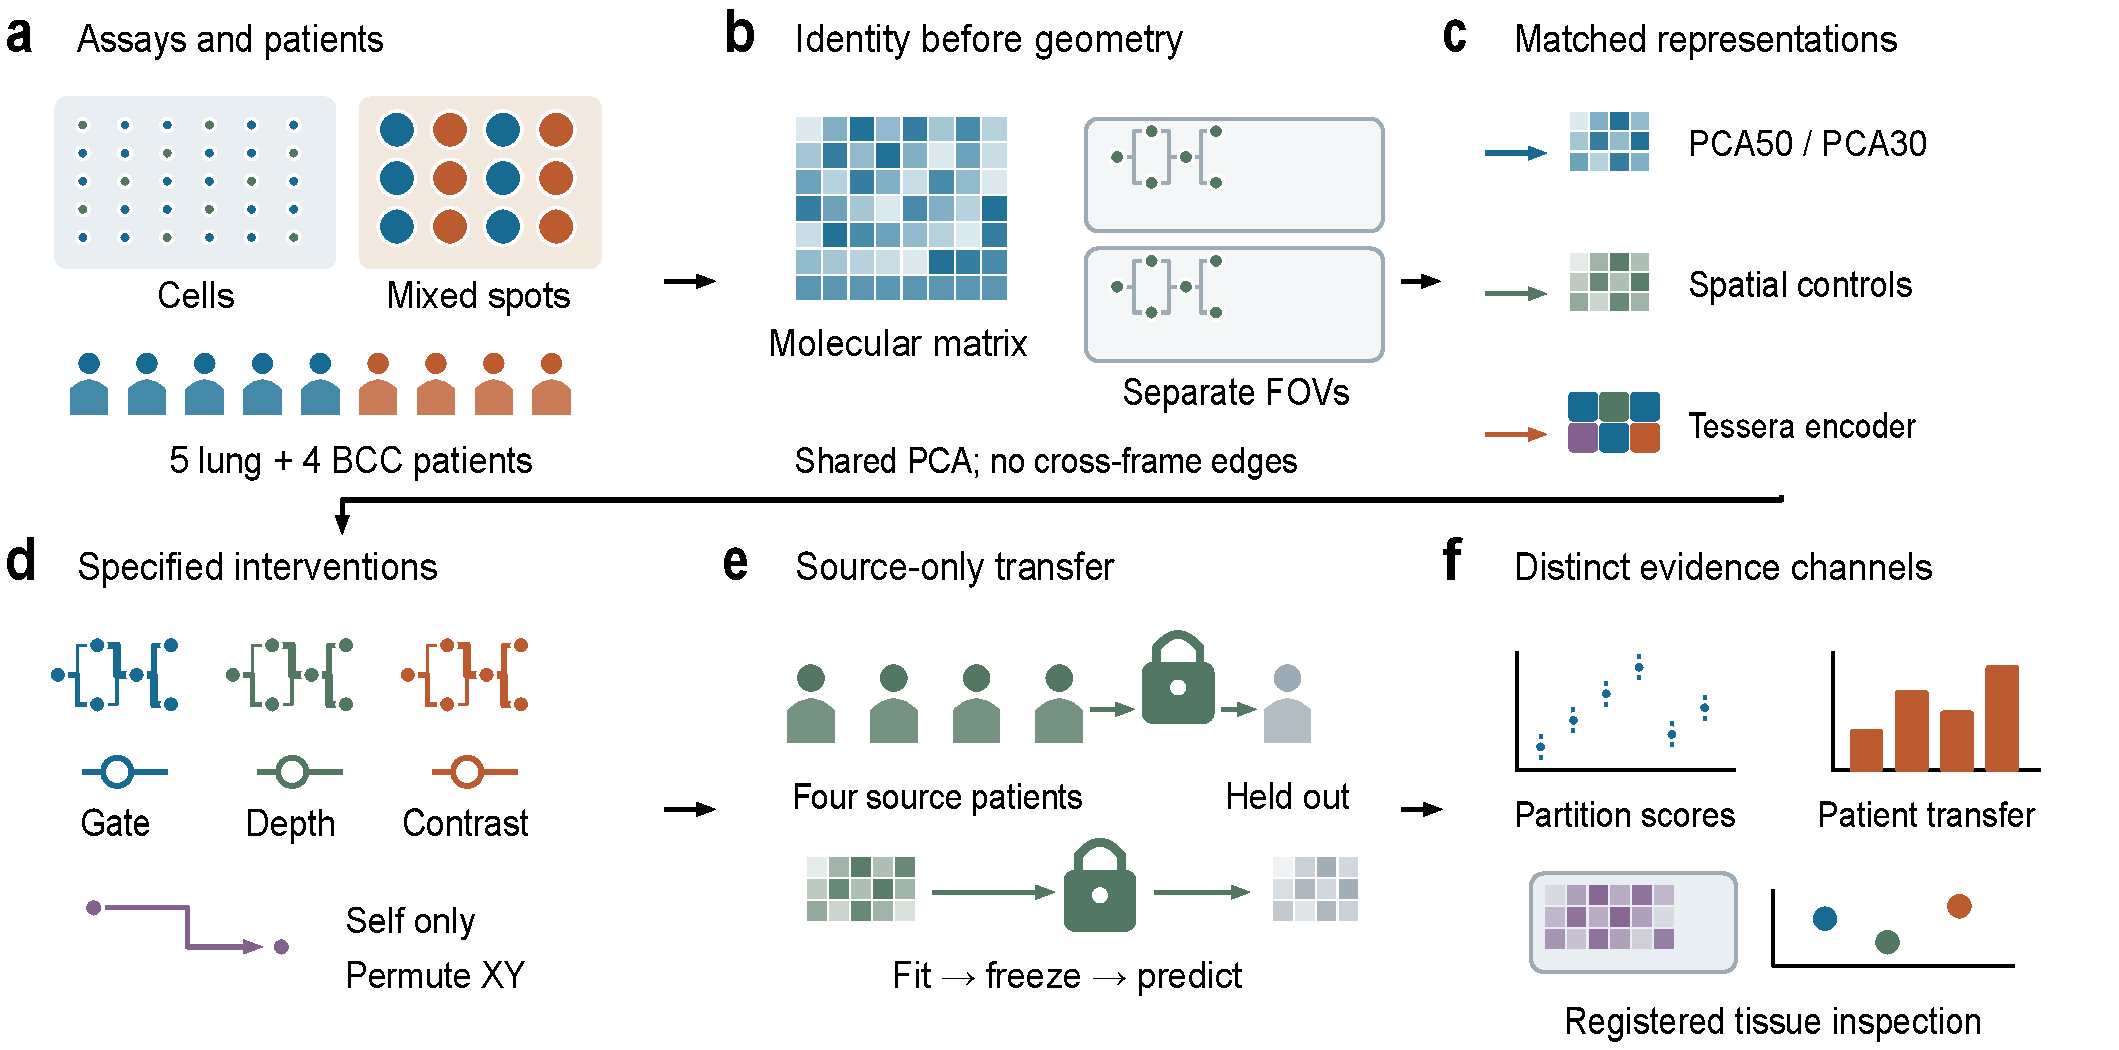
\includegraphics[width=\linewidth]{journal-figures/figure01-workflow.pdf}
\caption{Study design. (a) Assays and independent patients. (b) Molecular matrices and separate coordinate frames enter one common preprocessing. (c) Expression-only, simple spatial and learned representations form matched branches. (d) Component removals change one part of the encoder at a time. (e) In patient transfer, four source patients fit every transformation and weight before the fifth patient is mapped. (f) Partition, transfer and tissue-inspection readouts are reported separately. Icons are conceptual.}\label{fig:workflow}\end{figure}

\begin{table}[!htbp]\centering\small
\caption{Datasets analyzed. Counts refer to retained observations in the bounded inputs of at most 6,000 observations. Frames are coordinate identities, not patients. Class counts exclude missing labels.}\label{tab:inputs}
\begin{tabular}{lrrrrr}\toprule Object & Modeled & Labeled & Frames & Classes & Features\\\midrule
\tableinput ledgers/input_rows.tex
\bottomrule\end{tabular}\end{table}

\begin{figure}[!htbp]\centering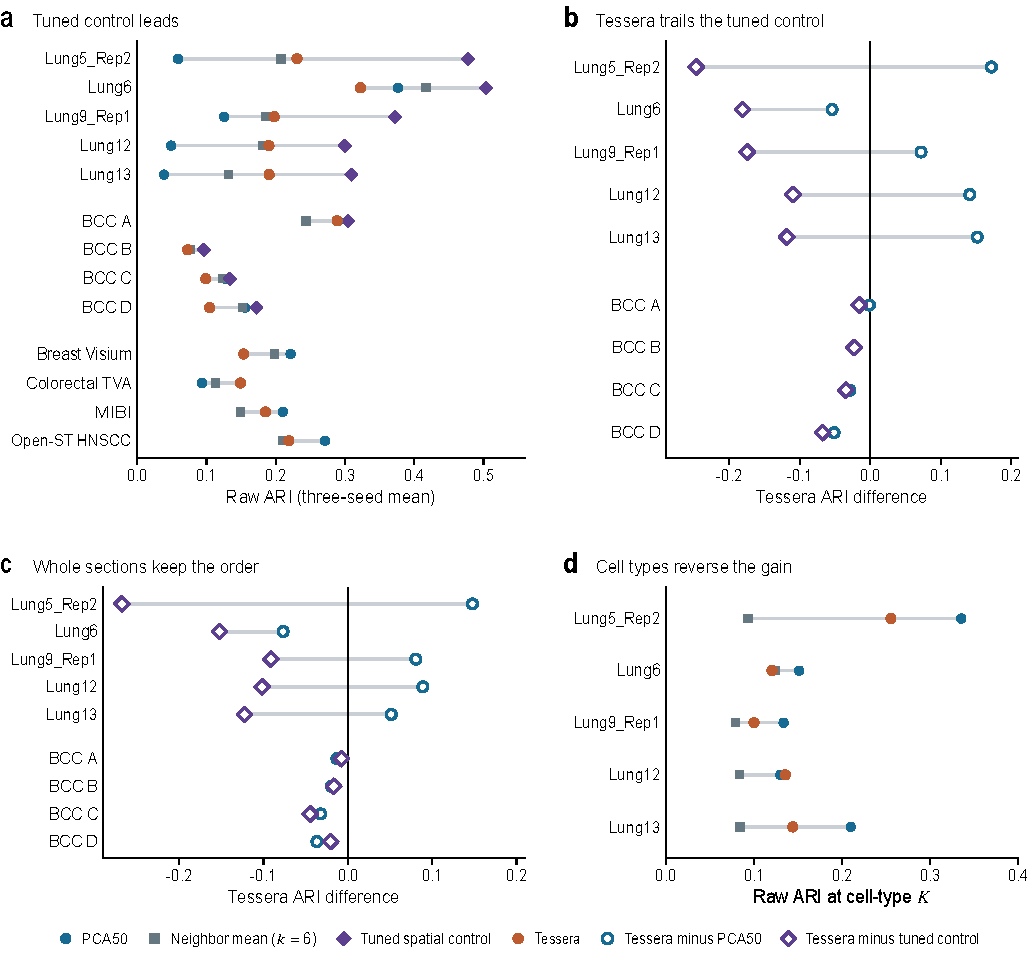
\includegraphics{journal-figures/figure03-comparison.pdf}
\caption{Tessera against expression-only, simple and tuned spatial controls. (a) Three-seed mean ARI per object; tuned controls are selected on other lung or BCC patients. (b) Bounded-field patient contrasts: Tessera minus PCA50 (open circles) and the nested control (open diamonds). (c) Uncapped whole-section sensitivity contrasts against PCA50 and fixed cohort-modal controls informed by the bounded analyses of the same patients. (d) Lung embeddings re-clustered at the cell-type cluster number and scored against supplied cell types.}\label{fig:comparison}\end{figure}

\begin{figure}[!htbp]\centering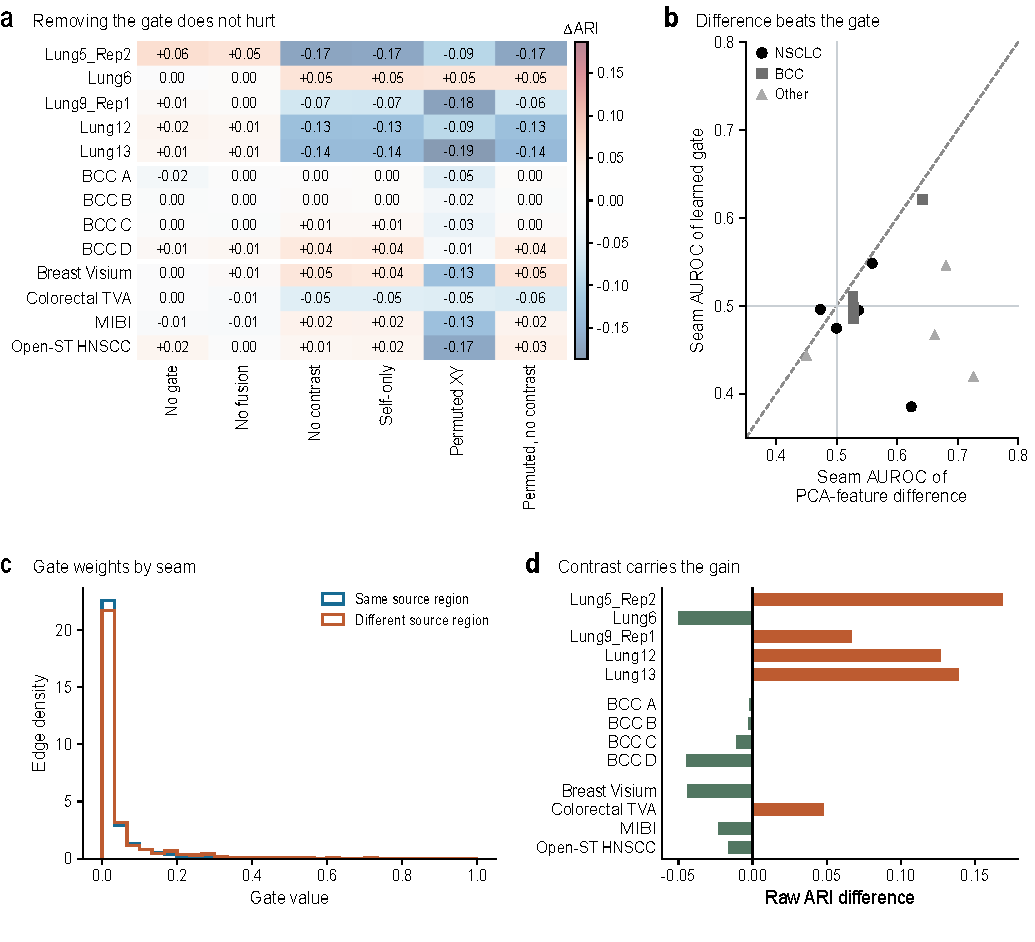
\includegraphics{journal-figures/figure04-ablations.pdf}
\caption{Which components carry the spatial effect. (a) Three-seed mean ARI of each control minus full Tessera; red favors the control. ``Permuted, no contrast'' trains on within-frame permuted coordinates without the contrastive term. (b) Seam discrimination by the last-layer gate versus by the plain PCA-feature difference on the same edges; points below the diagonal mean the gate is the weaker seam detector. (c) Last-layer gate distributions on edges within and across supplied regions in Lung5\_Rep2, seed 1. (d) Full Tessera minus the self-only encoder, the reference for the effect of measured geometry.}\label{fig:ablations}\end{figure}

\begin{figure}[!htbp]\centering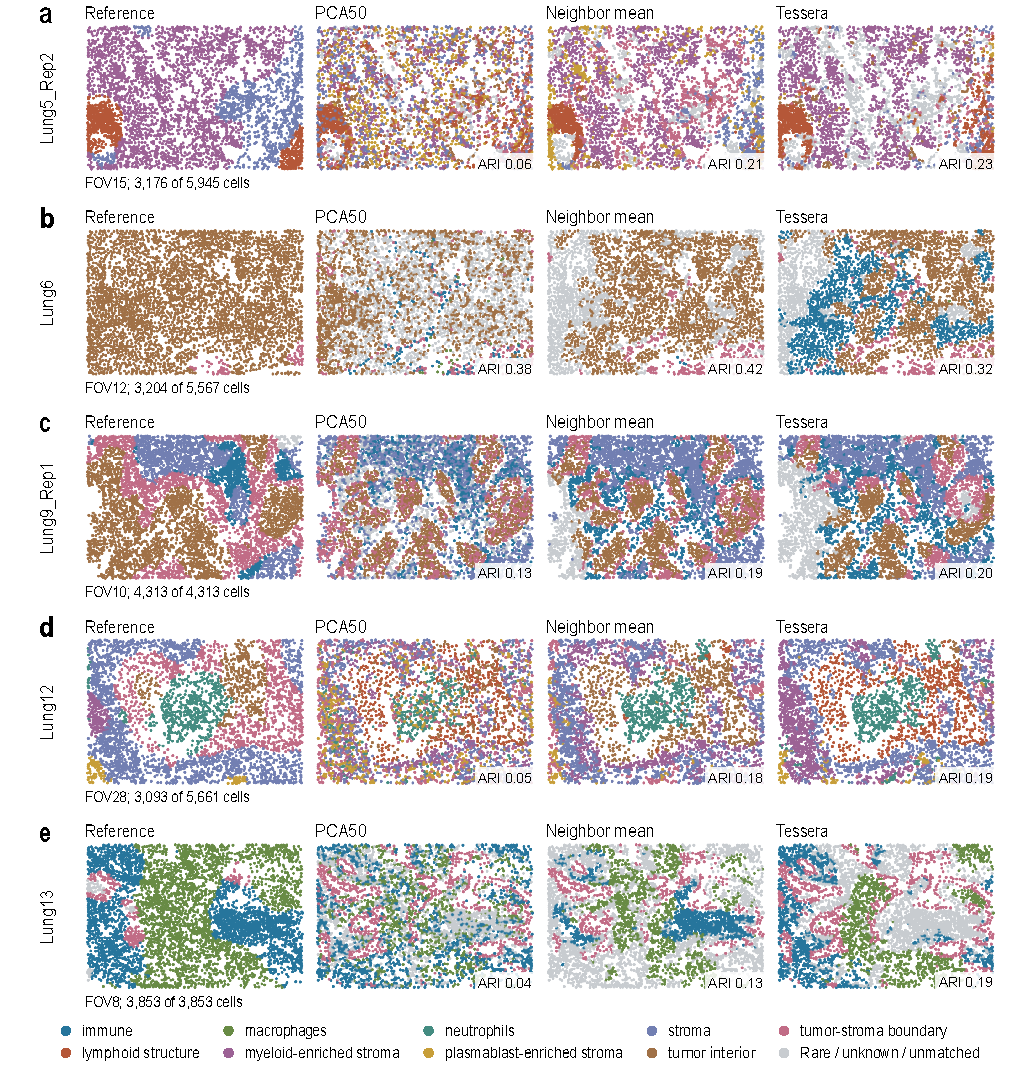
\includegraphics{journal-figures/figure05-nsclc-maps.pdf}
\caption{Lung display fields. Rows (a--e) show Lung5\_Rep2, Lung6, Lung9\_Rep1, Lung12 and Lung13; columns show supplied regions, PCA50, the six-neighbor mean and Tessera. Seed-1 clusters are color-matched only to reference classes with at least 1\% object-level prevalence; rare reference classes, unknown labels and unmatched clusters are gray. ARI badges use original predictions and all valid labels, averaged over three seeds and all retained fields. Lung6's display field is nearly one region.}\label{fig:lung}\end{figure}

\begin{figure}[!htbp]\centering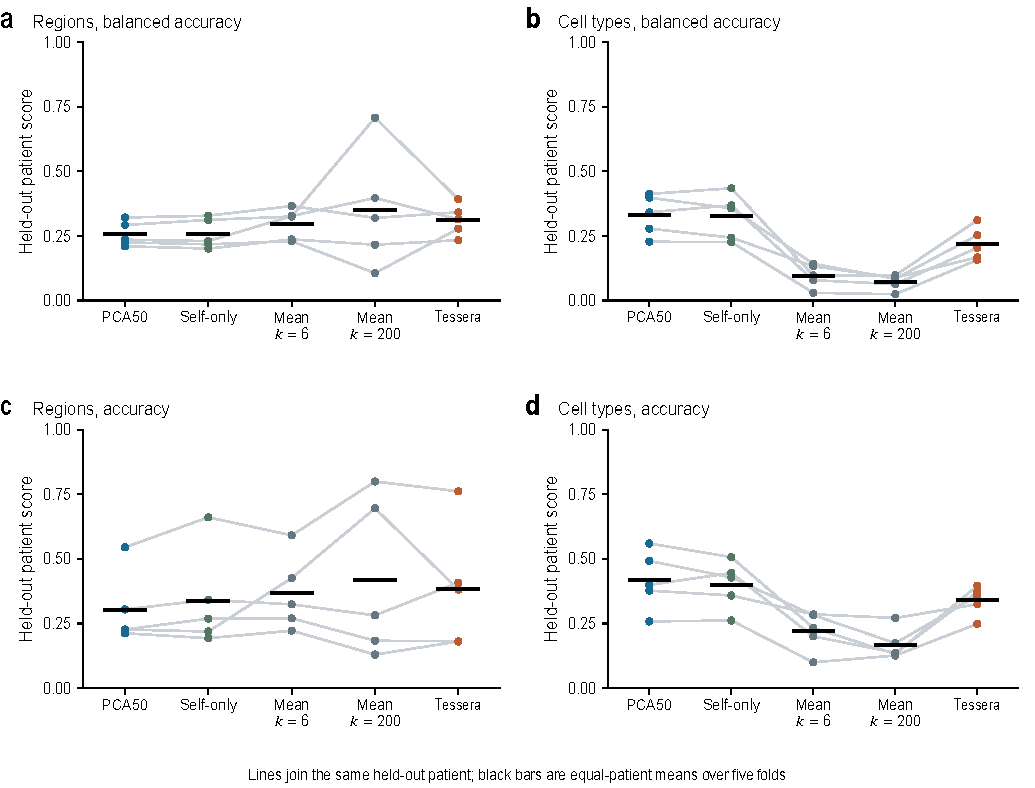
\includegraphics{journal-figures/figure10-patient-transfer.pdf}
\caption{Five patient-held-out NSCLC folds. (a, b) Region and cell-type balanced accuracy. (c, d) Accuracy. Four source patients fit scaling, PCA and the encoder; frozen parameters and source-category centroids map the held-out patient. Points are three-seed means for neural arms; fixed neighbor means (\(k=6,200\)) are deterministic descriptive controls, with \(k=200\) informed by earlier lung analyses, not fold-nested tuning. Lines join the same held-out patient; black bars are equal-patient means.}\label{fig:transfer}\end{figure}

\begin{figure}[!htbp]\centering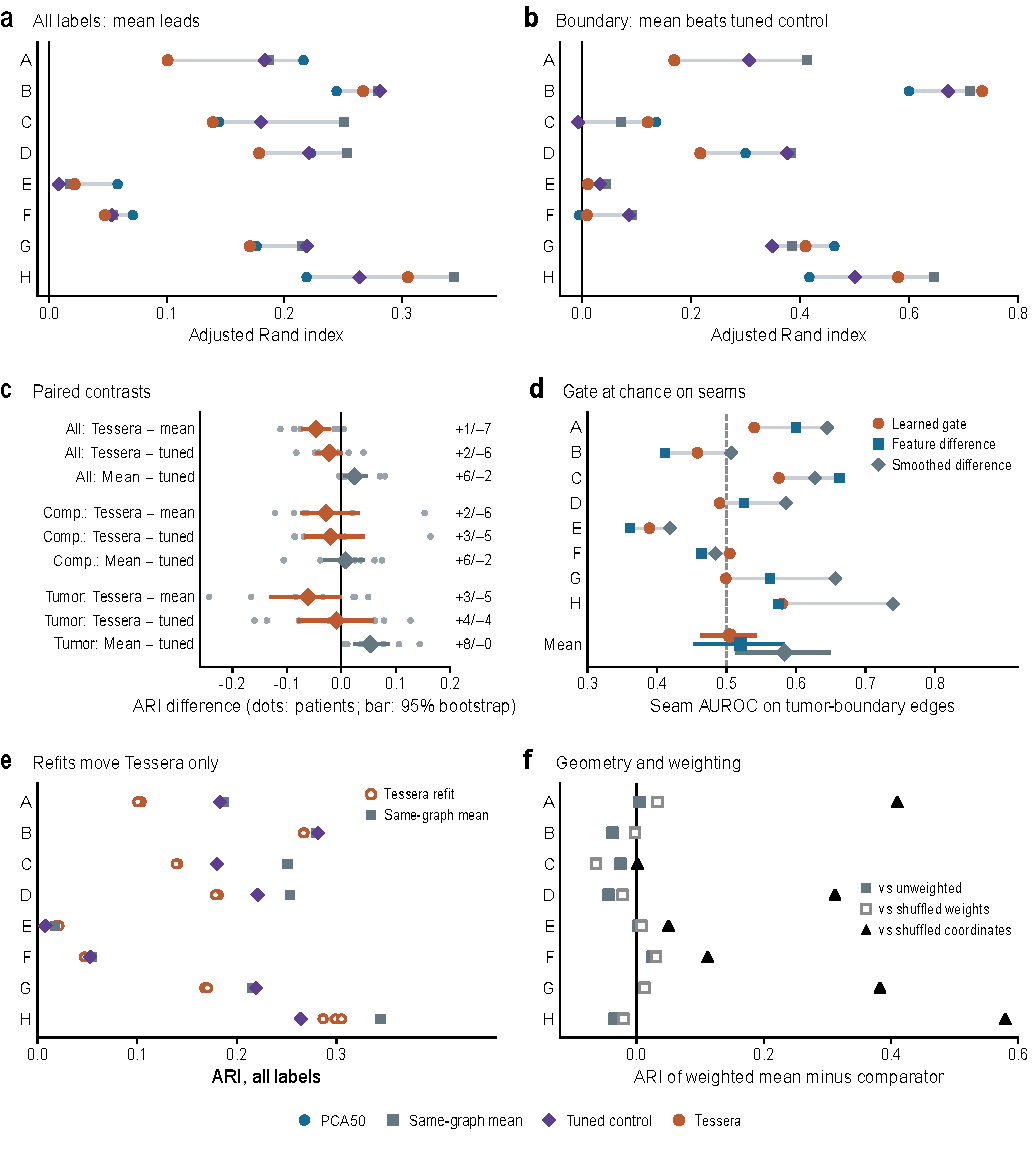
\includegraphics{journal-figures/figure15-external-cohort.pdf}
\caption{Independent pathologist-labelled cohort of eight HER2-positive breast tumors; rows A--H are patients. (a, b) Three-seed mean adjusted Rand index for all labels and for the tumor boundary: PCA50, the unweighted mean of neighbors on Tessera's graph, a tuned control selected on the other seven patients, and Tessera. (c) Paired differences for all labels (All), named compartments (Comp.) and the tumor boundary (Tumor); gray dots are patients, diamonds are means with 95\% bootstrap intervals, and the numbers count patients above and below zero. (d) Seam AUROC on tumor-boundary edges for the learned gate, the plain feature difference and the smoothed feature difference; the bottom rows give means with 95\% bootstrap intervals and the dashed line is chance. (e) Tessera's three replicate fits against the same-graph mean and the tuned control, all labels. (f) ARI of the weighted mean minus the unweighted mean, a mean with shuffled weights and a mean with shuffled coordinates, tumor boundary.}\label{fig:external}\end{figure}

\begin{figure}[!htbp]\centering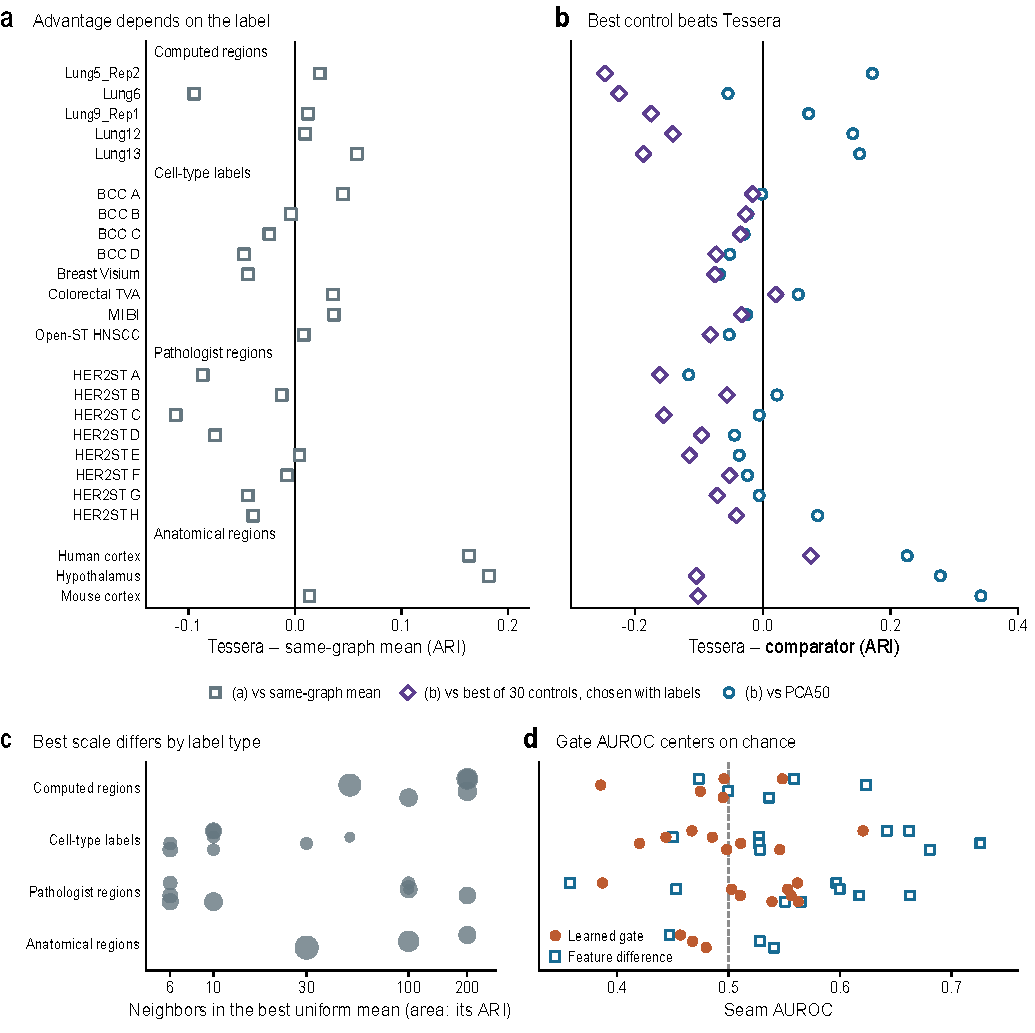
\includegraphics{journal-figures/figure17-tissue-landscape.pdf}
\caption{Twenty-four objects grouped by how the annotation was made: the 13 bounded objects, the eight independent patients and three further tissues. (a) Tessera minus the same-graph six-neighbor mean (ARI), which uses no label-based scale selection. (b) Tessera minus the best of 30 simple controls chosen with the test labels (diamonds) and minus PCA50 (circles). (c) Neighborhood size of the best uniform mean for each object; dot area is that mean's ARI. (d) Seam AUROC of the learned gate (filled) and the plain feature difference (open); the dashed line is chance.}\label{fig:landscape}\end{figure}
\end{document}
